\documentclass{amsart}
\usepackage{amssymb}
\usepackage{graphicx}
\usepackage[hidelinks]{hyperref}

% Compile with  pdflatex "\def\anonymous{}\documentclass{amsart}
\usepackage{amssymb}
\usepackage{graphicx}
\usepackage[hidelinks]{hyperref}

% Compile with  pdflatex "\def\anonymous{}\documentclass{amsart}
\usepackage{amssymb}
\usepackage{graphicx}
\usepackage[hidelinks]{hyperref}

% Compile with  pdflatex "\def\anonymous{}\documentclass{amsart}
\usepackage{amssymb}
\usepackage{graphicx}
\usepackage[hidelinks]{hyperref}

% Compile with  pdflatex "\def\anonymous{}\input{main}"  for the anonymized
% version required by the double-anonymous review of the journal.
\newif\ifanon
\ifdefined\anonymous\anontrue\fi

\newtheorem{theorem}{Theorem}[section]
\newtheorem{lemma}[theorem]{Lemma}
\newtheorem{proposition}[theorem]{Proposition}
\newtheorem{conjecture}[theorem]{Conjecture}
\theoremstyle{remark}
\newtheorem{remark}[theorem]{Remark}

\DeclareMathOperator{\age}{age}
\newcommand{\Iw}{\mathrm{I}_{4,\mathrm{wps}}}
\newcommand{\It}{\mathrm{I}_{4,\mathrm{term}}}
\newcommand{\Il}{\mathrm{I}_{4,\mathrm{loc}}}
\newcommand{\C}{\mathbb{C}}
\newcommand{\Z}{\mathbb{Z}}
\newcommand{\PP}{\mathbb{P}}
\newcommand{\A}{\mathbb{A}}
\newcommand{\zenodoID}{10.5281/zenodo.23387505}
\newcommand{\preprintURL}{https://github.com/creelie/fuzzy-guacamole/blob/main/preprintLiuFanoIndexConjecture/LiuFanoIndexConjecture.pdf}

\begin{document}

\title[Liu's conjecture on Fano indices]{A counterexample to Liu's conjecture on Fano indices in dimension four}

\ifanon\else
\author{Deep Bhattacharjee}
\address{Formerly, Electro-Gravitational Space Propulsion Laboratory (EGSPL),\newline Bhubaneswar, Odisha 751030, India}
\email{itsdeep@live.com}
\email{d.bhattacharjee@erl-forschung.de}
\author{Ushashi Bhattacharya}
\address{Formerly, National Taiwan University, Taipei 106319, Taiwan}
\email{rai.bhattacharya.in@gmail.com}
\thanks{Corresponding author: Deep Bhattacharjee. ORCID iDs: Deep Bhattacharjee 0000-0003-0466-750X; Ushashi Bhattacharya 0009-0002-2254-3914.}
\fi

\subjclass[2020]{Primary 14J32; Secondary 14B05, 14J45, 14M25}
\keywords{Fano index, weighted projective space, Calabi--Yau variety, log canonical singularity, index}

\begin{abstract}
We prove that Liu's conjecture on Fano indices fails in dimension four: $1389$ is the index of a terminal Calabi--Yau fourfold and of a four-dimensional log canonical singularity, but it is not the Fano index of any canonical weighted projective space of dimension four.
\end{abstract}

\maketitle

\section{Introduction}

We work over $\C$. For a well-formed weighted projective space $\PP(a_0,\dots,a_n)$ with canonical singularities, the Fano index is $q=a_0+\dots+a_n$. The \emph{index} of a Calabi--Yau variety $S$ (a normal projective variety with $K_S\sim_{\mathbb Q}0$) is the least $m\geq1$ with $mK_S\sim0$, and the index of a log canonical singularity $P\in Y$ is the least $m\geq1$ such that $mK_Y$ is Cartier at $P$. Following \cite[Definition~4.1]{Liu}, let
\begin{itemize}
\item $\mathrm{I}_{n,\mathrm{wps}}$ be the set of Fano indices of $n$-dimensional well-formed weighted projective spaces with canonical singularities, together with $\{1,\dots,n\}$;
\item $\mathrm{I}_{n,\mathrm{term}}$ be the set of indices of $n$-dimensional terminal Calabi--Yau varieties;
\item $\mathrm{I}_{n,\mathrm{loc}}$ be the set of indices of $n$-dimensional log canonical singularities.
\end{itemize}

\begin{conjecture}[{\cite[Conjecture~4.2]{Liu}}]\label{conj:liu}
$\mathrm{I}_{n,\mathrm{wps}}=\mathrm{I}_{n,\mathrm{term}}=\mathrm{I}_{n,\mathrm{loc}}$ for every $n\geq2$.
\end{conjecture}

Liu proves the conjecture for $n\leq3$ \cite[Proposition~4.3]{Liu} and computes $\Iw$ by an exhaustive search \cite[Theorem~4.4]{Liu}, \cite{LiuData}.

\begin{theorem}\label{thm:main}
$1389\in\It\cap\Il$ and $1389\notin\Iw$. In particular, Conjecture~\ref{conj:liu} fails for $n=4$.
\end{theorem}

The two memberships come from a symmetry of order $1389$ of one Calabi--Yau threefold, the hypersurface $X_{78}$ of $\PP(1,1,11,26,39)$ (Sections~\ref{sec:x}--\ref{sec:loc}). The non-membership is a finite statement about the $1{,}301{,}769{,}806$ partitions of $1389$ into five parts (Section~\ref{sec:wps}). It is proved in the Lean~4 kernel from a certificate of witnesses, together with the polynomial identities of Section~\ref{sec:x} (Section~\ref{sec:lean}). Figure~\ref{fig:roadmap} shows the plan of the proof.

\begin{figure}[ht]
\centering
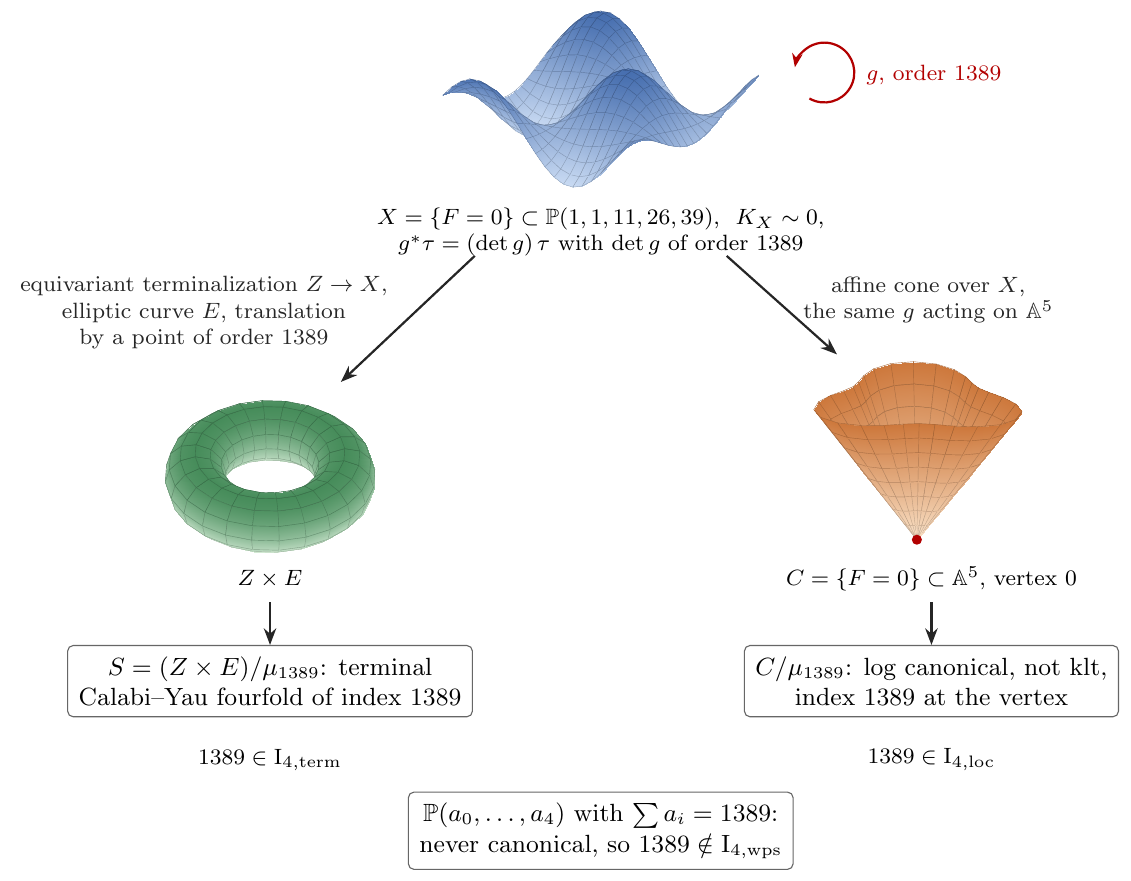
\includegraphics[width=\textwidth]{figures/fig_roadmap.png}
\caption{The plan of the proof. One symmetry $g$ of order $1389$ of the threefold $X$ gives a terminal Calabi--Yau fourfold of index $1389$ (Section~\ref{sec:term}) and a log canonical singularity of index $1389$ (Section~\ref{sec:loc}); no canonical weighted projective fourspace has Fano index $1389$ (Section~\ref{sec:wps}).}
\label{fig:roadmap}
\end{figure}

\begin{remark}\label{rem:literal}
Read literally, $\Il$ contains every positive integer: for $m\geq2$ the group $\mu_m$ acting on $\C^4$ with weights $(1,1,1,m-2)$ is free in codimension one, so $\C^4/\mu_m$ is klt, and $dx_1\wedge\dots\wedge dx_4$ has weight $m+1\equiv1\pmod m$, so its index is $m$ (by the argument in the proof of Proposition~\ref{prop:loc}). Since $3487\notin\Iw$ by \cite[Theorem~4.4]{Liu}, the literal reading fails at once, and the intended reading of $\mathrm{I}_{n,\mathrm{loc}}$ concerns log canonical singularities that are not klt. The singularity of Proposition~\ref{prop:loc} is log canonical and not klt, so Theorem~\ref{thm:main} holds for both readings.
\end{remark}

\section{The threefold}\label{sec:x}

Let $w=(w_0,\dots,w_4)=(1,1,11,26,39)$ and
\[
F=x_0^{77}x_1+x_1^{67}x_2+x_2^{7}x_0+x_3^3+x_4^2\in\C[x_0,\dots,x_4].
\]

\begin{lemma}\label{lem:F}
\begin{enumerate}
\item $F$ is quasi-homogeneous of degree $78=w_0+\dots+w_4$ for the weights $w$.
\item Any three of the $w_i$ are coprime.
\item The partial derivatives of $F$ have no common zero in $\C^5$ other than $0$.
\end{enumerate}
\end{lemma}

\begin{proof}
(1) and (2) are direct. For (3), let $x$ be a common zero; then $x_3=x_4=0$. With $\partial_i=\partial F/\partial x_i$,
\[
x_0\partial_0-77\,x_1\partial_1+5159\,x_2\partial_2=36114\,x_2^7x_0,
\]
since $x_0\partial_0=77x_0^{77}x_1+x_2^7x_0$, $x_1\partial_1=x_0^{77}x_1+67x_1^{67}x_2$ and $x_2\partial_2=x_1^{67}x_2+7x_2^7x_0$. Hence $x_2^7x_0=0$. If $x_2=0$, then $\partial_1=x_0^{77}$ and $\partial_2=x_1^{67}+7x_2^6x_0$ give $x_0=x_1=0$. If $x_0=0$, then $\partial_0=x_2^7$ gives $x_2=0$ and $\partial_2$ gives $x_1=0$.
\end{proof}

Let $C=\{F=0\}\subset\A^5$ and $X=\{F=0\}\subset\PP=\PP(1,1,11,26,39)$. By Lemma~\ref{lem:F}, $X$ is a quasi-smooth hypersurface of degree $78$; $\PP$ and $X$ are well formed \cite[6.10]{IF}. Hence $X$ has cyclic quotient singularities and $\omega_X\cong\mathcal O_X(78-\sum w_i)=\mathcal O_X$ \cite[6.14]{IF}. Quotient singularities are klt \cite[5.20]{KM}, and the discrepancies of a klt variety with Cartier canonical divisor are integers, so $X$ is a canonical Calabi--Yau threefold with $K_X\sim0$.

Fix a primitive $1389$th root of unity $\zeta$ and put $g=\operatorname{diag}(\zeta,\zeta^{1312},\zeta^{992},1,1)$.

\begin{lemma}\label{lem:g}
\begin{enumerate}
\item $F(gx)=F(x)$.
\item $\det g=\zeta^{2305}$ is a primitive $1389$th root of unity.
\item For $0<k<1389$, every fixed point $x\in\C^5$ of $g^k$ has $x_0=x_1=x_2=0$.
\end{enumerate}
\end{lemma}

\begin{proof}
(1) The monomials $x_0^{77}x_1$, $x_1^{67}x_2$ and $x_2^7x_0$ acquire the factors
\[
\zeta^{77+1312}=\zeta^{1389},\qquad\zeta^{67\cdot1312+992}=\zeta^{64\cdot1389},\qquad\zeta^{7\cdot992+1}=\zeta^{5\cdot1389}.
\] (2) $1389=3\cdot463$ and $2305=5\cdot461$ are coprime. (3) The integers $1$, $1312=2^5\cdot41$ and $992=2^5\cdot31$ are prime to $1389$, so $\zeta^k$, $\zeta^{1312k}$ and $\zeta^{992k}$ differ from $1$.
\end{proof}

The matrix $g$ commutes with the $\C^*$-action $t\cdot x=(t^{w_0}x_0,\dots,t^{w_4}x_4)$, so $G=\langle g\rangle\cong\mu_{1389}$ acts on $C$, on $\PP$ and on $X$. Let $\sigma$ be the Poincar\'e residue of $dx_0\wedge\dots\wedge dx_4/F$ along $C$; it generates $\omega_C$, and $g^*\sigma=\det(g)\,\sigma$ by Lemma~\ref{lem:g}(1).

\begin{lemma}\label{lem:omega}
$H^0(X,\omega_X)$ is spanned by a form $\tau$ with $g^*\tau=\det(g)\,\tau$.
\end{lemma}

\begin{proof}
Let $\xi=\sum w_ix_i\,\partial/\partial x_i$ and let $\rho\colon C\setminus\{0\}\to X$ be the quotient map. The $3$-form $\iota_\xi\sigma$ is $\C^*$-invariant, since $\sigma$ has weight $\sum w_i-78=0$, and $\iota_\xi\iota_\xi\sigma=0$. Let $X^\circ\subset X$ be the open set over which $\rho$ is a principal $\C^*$-bundle; its complement has codimension at least $2$ because $X$ is well formed. On $X^\circ$ there is a nowhere vanishing $3$-form $\tau$ with $\rho^*\tau=\iota_\xi\sigma$. As $\omega_X$ is reflexive, $\tau$ is a nowhere vanishing section of $\omega_X\cong\mathcal O_X$, so it spans $H^0(X,\omega_X)$. Since $g$ commutes with $\xi$ and with $\rho$, $g^*\tau=\det(g)\,\tau$.
\end{proof}

\section{A terminal Calabi--Yau fourfold of index 1389}\label{sec:term}

\begin{proposition}\label{prop:term}
$1389\in\It$.
\end{proposition}

\begin{proof}
By \cite[Proposition~2.2]{ETW} there is a $G$-equivariant projective birational morphism $\pi\colon Z\to X$ with $Z$ terminal and $K_Z=\pi^*K_X$. Then $\pi^*\tau$ is a nowhere vanishing section of $\omega_Z$, and $g^*\pi^*\tau=\det(g)\,\pi^*\tau$ by Lemma~\ref{lem:omega}. Let $E$ be an elliptic curve with a point $p$ of order $1389$, and let $G$ act on $Z\times E$ by $g(z,e)=(gz,e+p)$. The action is free, so $S=(Z\times E)/G$ is a terminal projective fourfold and $Z\times E\to S$ is \'etale. With $\eta$ a translation-invariant $1$-form on $E$, the form $\pi^*\tau\wedge\eta$ spans $H^0(Z\times E,\omega_{Z\times E})$ and $g$ multiplies it by $\det(g)$. For $m\geq1$, the sections of $\mathcal O_S(mK_S)$ are the $G$-invariant sections of $\omega_{Z\times E}^{\otimes m}$, so $H^0(S,\mathcal O_S(mK_S))\neq0$ if and only if $\det(g)^m=1$, that is, $1389\mid m$. As $K_S$ is numerically trivial, a nonzero section of $\mathcal O_S(mK_S)$ has no zeros, so $mK_S\sim0$ exactly when $1389\mid m$. This is the argument of \cite[Corollary~4.1]{ETW}. Hence $S$ is a terminal Calabi--Yau fourfold of index $1389$.
\end{proof}

\section{A log canonical singularity of index 1389}\label{sec:loc}

\begin{lemma}\label{lem:cone}
$C$ is normal and Gorenstein, log canonical, and not klt.
\end{lemma}

\begin{proof}
By Lemma~\ref{lem:F}(3), $C$ is a hypersurface whose only singular point is $0$, so $C$ is Gorenstein and, by Serre's criterion, normal; its local ring at $0$ is a domain, so $C$ is irreducible and no coordinate $x_j$ divides $F$.

Let $B\to\A^5$ be the weighted blow-up of $0$ with weights $w$. It is covered by the charts $U_i=\A^5/\mu_{w_i}$, where $\varphi_i\colon\A^5_y\to\A^5_x$ is $x_i=y_i^{w_i}$, $x_j=y_jy_i^{w_j}$ ($j\neq i$), and $\varepsilon\in\mu_{w_i}$ acts by $y_i\mapsto\varepsilon y_i$, $y_j\mapsto\varepsilon^{-w_j}y_j$. Quasi-homogeneity gives $F\circ\varphi_i=y_i^{78}F_i$, where $F_i$ is $F$ with $x_i$ replaced by $1$ and $x_j$ by $y_j$; it does not involve $y_i$. Let $S_i=\{F_i=0\}$ in the coordinates $y_j$, $j\neq i$. If $F_i$ and its derivatives vanish at $u$ (with $u_i=1$), the Euler identity $78F=\sum w_jx_j\partial_jF$ gives $\partial_iF(u)=0$, contradicting Lemma~\ref{lem:F}(3); so $S_i$ is smooth. The strict transform $W$ of $C$ is covered by $W_i=V_i/\mu_{w_i}$ with $V_i=\A^1_{y_i}\times S_i$, and the exceptional divisor $E_W=W\cap\pi^{-1}(0)$ is covered by $D_i/\mu_{w_i}$ with $D_i=\{0\}\times S_i$.

The action of $\mu_{w_i}$ on $V_i$ is free in codimension one. A non-identity $\varepsilon$ fixes no point with $y_i\neq0$. Its fixed points in $D_i$ satisfy $y_j=0$ for some $j\neq i$ with $\varepsilon^{w_j}\neq1$, which exists because the $w_j$ with $j\neq i$ are coprime; and $\{y_j=0\}$ contains no component of $S_i$ because $x_j\nmid F$. Hence $q_i\colon V_i\to W_i$ is \'etale in codimension one, $q_i^*K_{W_i}=K_{V_i}$ and $q_i^*E_W=D_i$. The pair $(V_i,D_i)$ is a smooth variety with a smooth divisor, hence log canonical, so $(W,E_W)$ is log canonical by \cite[5.20]{KM}.

The Jacobian of $\varphi_i$ is $w_iy_i^{\sum w_j-1}$, so
\[
\varphi_i^*(dx/F)=w_iy_i^{\sum w_j-1-78}\,dy/F_i=w_iy_i^{-1}\,dy/F_i,
\]
and the pullback of $\sigma$ to $V_i$ is $w_iy_i^{-1}$ times a generator of $\omega_{V_i}$. Thus the pullback of $\sigma$ to $W$ is a rational section of $\omega_W$ with divisor $-E_W$, that is, $K_W+E_W=\psi^*K_C$ for $\psi\colon W\to C$. By \cite[Lemma~2.30]{KM}, every divisor over $C$ has the same discrepancy for $C$ as for $(W,E_W)$. So $C$ is log canonical, and $E_W$ has discrepancy $-1$, so $C$ is not klt.
\end{proof}

\begin{figure}[ht]
\centering
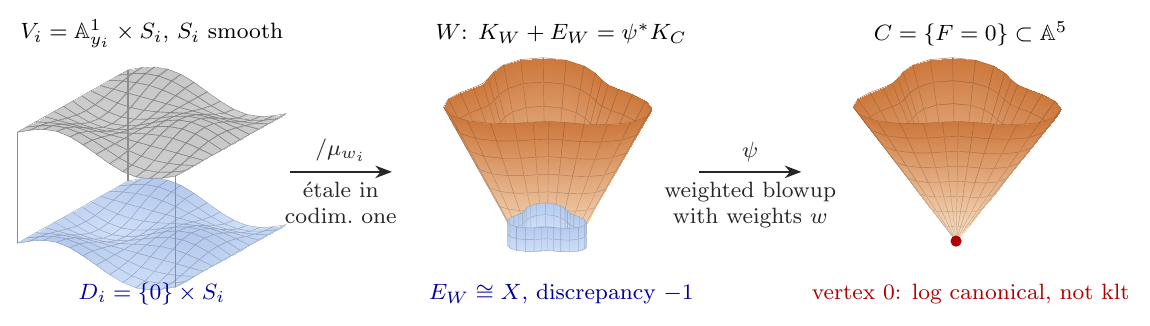
\includegraphics[width=\textwidth]{figures/fig_blowup.png}
\caption{The proof of Lemma~\ref{lem:cone}. The weighted blowup $\psi$ replaces the vertex of $C$ by $E_W\cong X$, and $K_W+E_W=\psi^*K_C$. On the chart $V_i$ the pair $(V_i,D_i)$ is a smooth variety with a smooth divisor, and $V_i\to W_i$ is a quotient by $\mu_{w_i}$ that is \'etale in codimension one.}
\label{fig:blowup}
\end{figure}

\begin{proposition}\label{prop:loc}
Let $Y=C/G$ and let $P\in Y$ be the image of $0$. Then $P\in Y$ is a four-dimensional log canonical singularity that is not klt and has index $1389$. In particular, $1389\in\Il$.
\end{proposition}

\begin{proof}
By Lemma~\ref{lem:g}(3), the fixed locus of $g^k$ on $C$ for $0<k<1389$ lies in the curve $\{x_0=x_1=x_2=0,\ x_3^3+x_4^2=0\}$. So $p\colon C\to Y$ is \'etale in codimension one, $K_C=p^*K_Y$, and $Y$ is log canonical and not klt by Lemma~\ref{lem:cone} and \cite[5.20]{KM}.

For $m\geq1$, the sections of $\mathcal O_Y(mK_Y)$ near $P$ are the $G$-invariant sections of $\omega_C^{\otimes m}$, that is, $f\sigma^m$ with $g^*f=\det(g)^{-m}f$. If $1389\mid m$, then $\sigma^m$ is invariant and generates. Conversely, if $mK_Y$ is Cartier at $P$ with generator $f\sigma^m$, then $f(0)\neq0$, and $g(0)=0$ gives $f(0)=\det(g)^{-m}f(0)$, so $1389\mid m$ by Lemma~\ref{lem:g}(2).
\end{proof}

\section{Weighted projective spaces of Fano index 1389}\label{sec:wps}

For $a=(a_0,\dots,a_4)\in\Z_{>0}^5$ with $q=\sum a_i$ and $k\in\Z$, put
\[
\age_a(k)=\sum_{i=0}^4\Big\{\frac{ka_i}{q}\Big\}=k-\sum_{i=0}^4\Big\lfloor\frac{ka_i}{q}\Big\rfloor.
\]
By Kasprzyk's criterion \cite[Proposition~2.5]{Kas}, a well-formed $\PP(a)$ has canonical singularities if and only if $\age_a(k)\in\{1,2,3\}$ for every $k\in\{2,\dots,q-2\}$.

\begin{lemma}\label{lem:witness}
Let $a\in\Z_{>0}^5$, $q=\sum a_i$, $k\in\Z$, and let $r_i\in\{0,\dots,q-1\}$ be the residue of $ka_i$ modulo $q$. If $r_i\geq1$ for $i=1,2,3,4$ and $r_1+r_2+r_3+r_4\leq q-1$, then $\age_a(q-k)=4$.
\end{lemma}

\begin{proof}
Since $\sum ka_i=kq$, we have $r_0\equiv-(r_1+\dots+r_4)\pmod q$, and $1\leq r_1+\dots+r_4\leq q-1$ gives $r_0=q-(r_1+\dots+r_4)\geq1$. All five residues are positive, so $\{(q-k)a_i/q\}=1-r_i/q$ and $\age_a(q-k)=5-\sum r_i/q=4$.
\end{proof}

\begin{proposition}\label{prop:cert}
Let $q=1389$. For all integers $1\leq a_4\leq a_3\leq a_2\leq a_1$ with $2a_1+a_2+a_3+a_4\leq q$ there is $k\in\{2,\dots,q-2\}$ such that the residues $r_i$ of $ka_i$ modulo $q$ satisfy $r_1,\dots,r_4\geq1$ and $r_1+r_2+r_3+r_4\leq q-1$.
\end{proposition}

\begin{proof}
The proof is a finite verification, carried out in the Lean kernel (Section~\ref{sec:lean}). For $t=(t_1,\dots,t_4)$ with $t_4\leq t_3\leq t_2\leq t_1$ let $x_i=1+8t_i$ and let $Q_t$ be the box $\prod_i\{x_i,\dots,x_i+7\}$. Every admissible $(a_1,\dots,a_4)$ lies in $Q_t$ for $t_i=\lfloor(a_i-1)/8\rfloor$, and then $2x_1+x_2+x_3+x_4\leq q$. There are $368{,}253$ such $t$. For each of them the certificate lists values of $k$, $2{,}624{,}293$ in all and at most $70$ per box; one value suffices for $231{,}139$ boxes. The condition on $k$ is equivalent to
\begin{equation}\label{eq:test}
\sum_{i=1}^4\big(((ka_i+q-1)\bmod q)+1\big)\leq q-1,
\end{equation}
because $((ka+q-1)\bmod q)+1$ equals the residue of $ka$ when that residue is positive and equals $q$ otherwise. Write $a_i=x_i+\delta_i$ with $0\leq\delta_i\leq7$ and $c_i=(kx_i+q-1)\bmod q$. Then $(ka_i+q-1)\bmod q=c_i+k\delta_i-q\lfloor(c_i+k\delta_i)/q\rfloor$ and
\[
\Big\lfloor\frac{c_i+k\delta_i}{q}\Big\rfloor=\#\Big\{j\geq1:\ \delta_i\geq\Big\lceil\frac{jq-c_i}{k}\Big\rceil\Big\},
\]
a sum of at most $\lfloor(c_i+7k)/q\rfloor$ indicator functions of $\delta_i$. The checker stores the $8^4$ points of a box in $17$-bit fields of one natural number and evaluates \eqref{eq:test}, the order conditions and the linear condition for all of them by additions, multiplications by integers, shifts and bitwise conjunctions; a box passes when every admissible point satisfies \eqref{eq:test} for some listed $k$. The soundness of the checker, namely that a passing box has this property, is proved in Lean, and the kernel evaluates the checker on all boxes.
\end{proof}

\begin{figure}[ht]
\centering
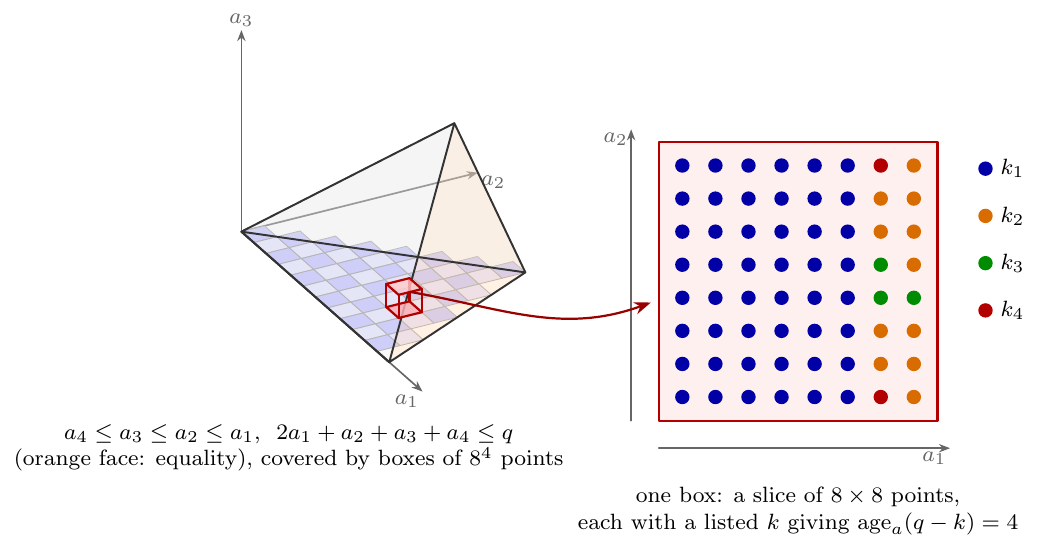
\includegraphics[width=\textwidth]{figures/fig_boxes.png}
\caption{The certificate of Proposition~\ref{prop:cert}. The sorted weights with $2a_1+a_2+a_3+a_4\leq q$ are covered by boxes of $8^4$ points (drawn in the coordinates $a_1,a_2,a_3$). For each box the certificate lists values of $k$; every point of the box is served by one of them. The right panel shows the points of one slice of one box, coloured by the listed value that serves them.}
\label{fig:boxes}
\end{figure}

\begin{theorem}\label{thm:wps}
Every $a\in\Z_{>0}^5$ with $\sum a_i=1389$ has $\age_a(k)=4$ for some $k\in\{2,\dots,1387\}$. Hence no well-formed weighted projective space $\PP(a_0,\dots,a_4)$ of Fano index $1389$ has canonical singularities, and $1389\notin\Iw$.
\end{theorem}

\begin{proof}
Order the weights so that $a_0\geq a_1\geq\dots\geq a_4$. Then $2a_1+a_2+a_3+a_4\leq a_0+\dots+a_4=1389$. Proposition~\ref{prop:cert} gives $k\in\{2,\dots,1387\}$, and Lemma~\ref{lem:witness} gives $\age_a(1389-k)=4$ with $1389-k\in\{2,\dots,1387\}$. Kasprzyk's criterion excludes canonical singularities, and $1389>4$.
\end{proof}

\begin{proof}[Proof of Theorem~\textup{\ref{thm:main}}]
Combine Propositions~\ref{prop:term} and~\ref{prop:loc} with Theorem~\ref{thm:wps}.
\end{proof}

\begin{remark}
Since $\varphi(1389)=924\leq984$, the number $1389$ lies in the set $\{m:\varphi(m)\leq984\}$ that contains $\Iw$ by \cite[Theorem~4.4]{Liu}; it is one of the elements of the set $\mathrm J_4$ of \cite[Section~4]{Liu}. Theorem~\ref{thm:wps} agrees with the list \cite{LiuData}. The neighbouring index $1383$ lies in $\Iw$: $\PP(674,461,195,35,18)$ is well formed and passes Kasprzyk's criterion.
\end{remark}

\section{Formal verification}\label{sec:lean}

The finite and algebraic parts of the proof are formalized in Lean~4 with its mathematical library \cite{Lean,Mathlib}. In the formalization the set $\Iw$ is defined as the union of $\{1,2,3,4\}$ with the sums $\sum a_i$ over the well-formed $a\in\Z_{>0}^5$ that satisfy Kasprzyk's criterion. The formal statements are Lemma~\ref{lem:F}, Lemma~\ref{lem:g}, Proposition~\ref{prop:cert}, the first part of Theorem~\ref{thm:wps}, and the statement $1389\notin\Iw$. The kernel checks every proof, and each of these theorems depends only on the axioms of propositional extensionality, choice and quotient soundness.

The certificate of Proposition~\ref{prop:cert} is split into $4{,}022$ statements, each asserting that the checker accepts one list of boxes. Each statement is closed by evaluating the checker in the kernel, so no compiled code is trusted; checking all of them takes about $15$ minutes on four cores. The steps that rest on the literature, namely Kasprzyk's criterion, the results of \cite{IF} and \cite{ETW}, and the singularity theory of Sections~\ref{sec:x}--\ref{sec:loc}, are proved in the text and not formalized, since the library does not yet contain weighted projective spaces or discrepancies.

Independently of the formalization, programs in C, C++, Julia and Python enumerate all $1{,}301{,}769{,}806$ partitions of $1389$ into five parts, test Kasprzyk's criterion on the $874{,}763{,}737$ well-formed ones, and find no canonical one. The same enumeration for $q=1383$ finds $\PP(674,461,195,35,18)$.

\section*{Acknowledgements}
The authors used the generative AI tool Claude (Anthropic), through Claude Code, to assist with the proofs, the Lean formalization, the computations and the preparation of this article. The authors reviewed and edited the content and take full responsibility for it.

\section*{Competing interests}
None.

\section*{Funding}
None.

\section*{Data availability}
\begingroup\raggedright
\ifanon
The computations and the Lean formalization were carried out by the authors with the help of AI assistance (Claude, Anthropic). The Lean formalization, the certificate generator and the search programs are supplied with the submission.\par
\else
Deep Bhattacharjee computed the Lean formalization and the Julia, C, C++, shell and Python computations with the help of AI assistance (Claude, Anthropic). The Lean formalization of the finite and algebraic parts of the proof, together with the certificate generator and the search programs, is archived at Zenodo \cite{archive}, doi:\href{https://doi.org/\zenodoID}{\zenodoID}. The paper is available at \url{\preprintURL}.\par
\fi
\endgroup

\begin{thebibliography}{99}
\raggedright

\ifanon\else
\bibitem{archive}
D.~Bhattacharjee and U.~Bhattacharya, \emph{A counterexample to Liu's conjecture on Fano indices in dimension four: Lean formalization and programs}, Zenodo, 2026, doi:\href{https://doi.org/\zenodoID}{\zenodoID}.
\fi

\bibitem{Mathlib}
The mathlib Community, \emph{The Lean mathematical library}, in: Proceedings of the 9th ACM SIGPLAN International Conference on Certified Programs and Proofs (CPP 2020), ACM, 2020, pp.~367--381, doi:\href{https://doi.org/10.1145/3372885.3373824}{10.1145/3372885.3373824}.

\bibitem{ETW}
L.~Esser, B.~Totaro and C.~Wang, \emph{Calabi--Yau varieties of large index}, Algebr. Geom., to appear; arXiv:2209.04597.

\bibitem{IF}
A.~R.~Iano-Fletcher, \emph{Working with weighted complete intersections}, in: Explicit birational geometry of 3-folds, London Math. Soc. Lecture Note Ser. 281, Cambridge Univ. Press, Cambridge, 2000, pp.~101--174, doi:\href{https://doi.org/10.1017/CBO9780511758942.005}{10.1017/CBO9780511758942.005}.

\bibitem{Kas}
A.~M.~Kasprzyk, \emph{Classifying terminal weighted projective space}, arXiv:1304.3029.

\bibitem{KM}
J.~Koll\'ar and S.~Mori, \emph{Birational geometry of algebraic varieties}, Cambridge Tracts in Math. 134, Cambridge Univ. Press, Cambridge, 1998, doi:\href{https://doi.org/10.1017/CBO9780511662560}{10.1017/CBO9780511662560}.

\bibitem{Liu}
H.~Liu, \emph{On Fano indices of weighted projective spaces}, arXiv:2608.03434v3, 2026.

\bibitem{LiuData}
H.~Liu, \emph{Fano indices of four-dimensional canonical weighted projective spaces} (data and code), Zenodo, doi:\href{https://doi.org/10.5281/zenodo.21806548}{10.5281/zenodo.21806548}.

\bibitem{Lean}
L.~de~Moura and S.~Ullrich, \emph{The Lean~4 theorem prover and programming language}, in: Automated Deduction -- CADE 28, Lecture Notes in Comput. Sci. 12699, Springer, 2021, pp.~625--635, doi:\href{https://doi.org/10.1007/978-3-030-79876-5_37}{10.1007/978-3-030-79876-5\_37}.

\end{thebibliography}

\end{document}
"  for the anonymized
% version required by the double-anonymous review of the journal.
\newif\ifanon
\ifdefined\anonymous\anontrue\fi

\newtheorem{theorem}{Theorem}[section]
\newtheorem{lemma}[theorem]{Lemma}
\newtheorem{proposition}[theorem]{Proposition}
\newtheorem{conjecture}[theorem]{Conjecture}
\theoremstyle{remark}
\newtheorem{remark}[theorem]{Remark}

\DeclareMathOperator{\age}{age}
\newcommand{\Iw}{\mathrm{I}_{4,\mathrm{wps}}}
\newcommand{\It}{\mathrm{I}_{4,\mathrm{term}}}
\newcommand{\Il}{\mathrm{I}_{4,\mathrm{loc}}}
\newcommand{\C}{\mathbb{C}}
\newcommand{\Z}{\mathbb{Z}}
\newcommand{\PP}{\mathbb{P}}
\newcommand{\A}{\mathbb{A}}
\newcommand{\zenodoID}{10.5281/zenodo.23387505}
\newcommand{\preprintURL}{https://github.com/creelie/fuzzy-guacamole/blob/main/preprintLiuFanoIndexConjecture/LiuFanoIndexConjecture.pdf}

\begin{document}

\title[Liu's conjecture on Fano indices]{A counterexample to Liu's conjecture on Fano indices in dimension four}

\ifanon\else
\author{Deep Bhattacharjee}
\address{Formerly, Electro-Gravitational Space Propulsion Laboratory (EGSPL),\newline Bhubaneswar, Odisha 751030, India}
\email{itsdeep@live.com}
\email{d.bhattacharjee@erl-forschung.de}
\author{Ushashi Bhattacharya}
\address{Formerly, National Taiwan University, Taipei 106319, Taiwan}
\email{rai.bhattacharya.in@gmail.com}
\thanks{Corresponding author: Deep Bhattacharjee. ORCID iDs: Deep Bhattacharjee 0000-0003-0466-750X; Ushashi Bhattacharya 0009-0002-2254-3914.}
\fi

\subjclass[2020]{Primary 14J32; Secondary 14B05, 14J45, 14M25}
\keywords{Fano index, weighted projective space, Calabi--Yau variety, log canonical singularity, index}

\begin{abstract}
We prove that Liu's conjecture on Fano indices fails in dimension four: $1389$ is the index of a terminal Calabi--Yau fourfold and of a four-dimensional log canonical singularity, but it is not the Fano index of any canonical weighted projective space of dimension four.
\end{abstract}

\maketitle

\section{Introduction}

We work over $\C$. For a well-formed weighted projective space $\PP(a_0,\dots,a_n)$ with canonical singularities, the Fano index is $q=a_0+\dots+a_n$. The \emph{index} of a Calabi--Yau variety $S$ (a normal projective variety with $K_S\sim_{\mathbb Q}0$) is the least $m\geq1$ with $mK_S\sim0$, and the index of a log canonical singularity $P\in Y$ is the least $m\geq1$ such that $mK_Y$ is Cartier at $P$. Following \cite[Definition~4.1]{Liu}, let
\begin{itemize}
\item $\mathrm{I}_{n,\mathrm{wps}}$ be the set of Fano indices of $n$-dimensional well-formed weighted projective spaces with canonical singularities, together with $\{1,\dots,n\}$;
\item $\mathrm{I}_{n,\mathrm{term}}$ be the set of indices of $n$-dimensional terminal Calabi--Yau varieties;
\item $\mathrm{I}_{n,\mathrm{loc}}$ be the set of indices of $n$-dimensional log canonical singularities.
\end{itemize}

\begin{conjecture}[{\cite[Conjecture~4.2]{Liu}}]\label{conj:liu}
$\mathrm{I}_{n,\mathrm{wps}}=\mathrm{I}_{n,\mathrm{term}}=\mathrm{I}_{n,\mathrm{loc}}$ for every $n\geq2$.
\end{conjecture}

Liu proves the conjecture for $n\leq3$ \cite[Proposition~4.3]{Liu} and computes $\Iw$ by an exhaustive search \cite[Theorem~4.4]{Liu}, \cite{LiuData}.

\begin{theorem}\label{thm:main}
$1389\in\It\cap\Il$ and $1389\notin\Iw$. In particular, Conjecture~\ref{conj:liu} fails for $n=4$.
\end{theorem}

The two memberships come from a symmetry of order $1389$ of one Calabi--Yau threefold, the hypersurface $X_{78}$ of $\PP(1,1,11,26,39)$ (Sections~\ref{sec:x}--\ref{sec:loc}). The non-membership is a finite statement about the $1{,}301{,}769{,}806$ partitions of $1389$ into five parts (Section~\ref{sec:wps}). It is proved in the Lean~4 kernel from a certificate of witnesses, together with the polynomial identities of Section~\ref{sec:x} (Section~\ref{sec:lean}). Figure~\ref{fig:roadmap} shows the plan of the proof.

\begin{figure}[ht]
\centering
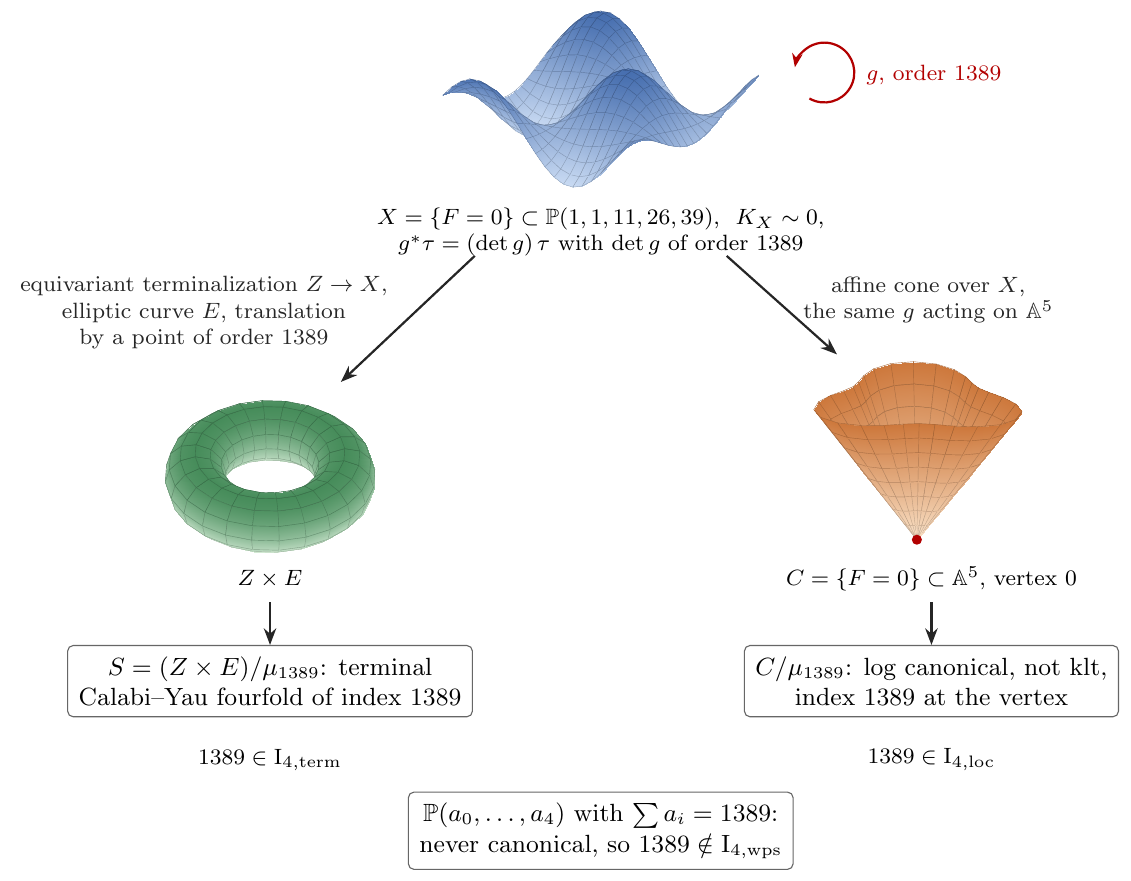
\includegraphics[width=\textwidth]{figures/fig_roadmap.png}
\caption{The plan of the proof. One symmetry $g$ of order $1389$ of the threefold $X$ gives a terminal Calabi--Yau fourfold of index $1389$ (Section~\ref{sec:term}) and a log canonical singularity of index $1389$ (Section~\ref{sec:loc}); no canonical weighted projective fourspace has Fano index $1389$ (Section~\ref{sec:wps}).}
\label{fig:roadmap}
\end{figure}

\begin{remark}\label{rem:literal}
Read literally, $\Il$ contains every positive integer: for $m\geq2$ the group $\mu_m$ acting on $\C^4$ with weights $(1,1,1,m-2)$ is free in codimension one, so $\C^4/\mu_m$ is klt, and $dx_1\wedge\dots\wedge dx_4$ has weight $m+1\equiv1\pmod m$, so its index is $m$ (by the argument in the proof of Proposition~\ref{prop:loc}). Since $3487\notin\Iw$ by \cite[Theorem~4.4]{Liu}, the literal reading fails at once, and the intended reading of $\mathrm{I}_{n,\mathrm{loc}}$ concerns log canonical singularities that are not klt. The singularity of Proposition~\ref{prop:loc} is log canonical and not klt, so Theorem~\ref{thm:main} holds for both readings.
\end{remark}

\section{The threefold}\label{sec:x}

Let $w=(w_0,\dots,w_4)=(1,1,11,26,39)$ and
\[
F=x_0^{77}x_1+x_1^{67}x_2+x_2^{7}x_0+x_3^3+x_4^2\in\C[x_0,\dots,x_4].
\]

\begin{lemma}\label{lem:F}
\begin{enumerate}
\item $F$ is quasi-homogeneous of degree $78=w_0+\dots+w_4$ for the weights $w$.
\item Any three of the $w_i$ are coprime.
\item The partial derivatives of $F$ have no common zero in $\C^5$ other than $0$.
\end{enumerate}
\end{lemma}

\begin{proof}
(1) and (2) are direct. For (3), let $x$ be a common zero; then $x_3=x_4=0$. With $\partial_i=\partial F/\partial x_i$,
\[
x_0\partial_0-77\,x_1\partial_1+5159\,x_2\partial_2=36114\,x_2^7x_0,
\]
since $x_0\partial_0=77x_0^{77}x_1+x_2^7x_0$, $x_1\partial_1=x_0^{77}x_1+67x_1^{67}x_2$ and $x_2\partial_2=x_1^{67}x_2+7x_2^7x_0$. Hence $x_2^7x_0=0$. If $x_2=0$, then $\partial_1=x_0^{77}$ and $\partial_2=x_1^{67}+7x_2^6x_0$ give $x_0=x_1=0$. If $x_0=0$, then $\partial_0=x_2^7$ gives $x_2=0$ and $\partial_2$ gives $x_1=0$.
\end{proof}

Let $C=\{F=0\}\subset\A^5$ and $X=\{F=0\}\subset\PP=\PP(1,1,11,26,39)$. By Lemma~\ref{lem:F}, $X$ is a quasi-smooth hypersurface of degree $78$; $\PP$ and $X$ are well formed \cite[6.10]{IF}. Hence $X$ has cyclic quotient singularities and $\omega_X\cong\mathcal O_X(78-\sum w_i)=\mathcal O_X$ \cite[6.14]{IF}. Quotient singularities are klt \cite[5.20]{KM}, and the discrepancies of a klt variety with Cartier canonical divisor are integers, so $X$ is a canonical Calabi--Yau threefold with $K_X\sim0$.

Fix a primitive $1389$th root of unity $\zeta$ and put $g=\operatorname{diag}(\zeta,\zeta^{1312},\zeta^{992},1,1)$.

\begin{lemma}\label{lem:g}
\begin{enumerate}
\item $F(gx)=F(x)$.
\item $\det g=\zeta^{2305}$ is a primitive $1389$th root of unity.
\item For $0<k<1389$, every fixed point $x\in\C^5$ of $g^k$ has $x_0=x_1=x_2=0$.
\end{enumerate}
\end{lemma}

\begin{proof}
(1) The monomials $x_0^{77}x_1$, $x_1^{67}x_2$ and $x_2^7x_0$ acquire the factors
\[
\zeta^{77+1312}=\zeta^{1389},\qquad\zeta^{67\cdot1312+992}=\zeta^{64\cdot1389},\qquad\zeta^{7\cdot992+1}=\zeta^{5\cdot1389}.
\] (2) $1389=3\cdot463$ and $2305=5\cdot461$ are coprime. (3) The integers $1$, $1312=2^5\cdot41$ and $992=2^5\cdot31$ are prime to $1389$, so $\zeta^k$, $\zeta^{1312k}$ and $\zeta^{992k}$ differ from $1$.
\end{proof}

The matrix $g$ commutes with the $\C^*$-action $t\cdot x=(t^{w_0}x_0,\dots,t^{w_4}x_4)$, so $G=\langle g\rangle\cong\mu_{1389}$ acts on $C$, on $\PP$ and on $X$. Let $\sigma$ be the Poincar\'e residue of $dx_0\wedge\dots\wedge dx_4/F$ along $C$; it generates $\omega_C$, and $g^*\sigma=\det(g)\,\sigma$ by Lemma~\ref{lem:g}(1).

\begin{lemma}\label{lem:omega}
$H^0(X,\omega_X)$ is spanned by a form $\tau$ with $g^*\tau=\det(g)\,\tau$.
\end{lemma}

\begin{proof}
Let $\xi=\sum w_ix_i\,\partial/\partial x_i$ and let $\rho\colon C\setminus\{0\}\to X$ be the quotient map. The $3$-form $\iota_\xi\sigma$ is $\C^*$-invariant, since $\sigma$ has weight $\sum w_i-78=0$, and $\iota_\xi\iota_\xi\sigma=0$. Let $X^\circ\subset X$ be the open set over which $\rho$ is a principal $\C^*$-bundle; its complement has codimension at least $2$ because $X$ is well formed. On $X^\circ$ there is a nowhere vanishing $3$-form $\tau$ with $\rho^*\tau=\iota_\xi\sigma$. As $\omega_X$ is reflexive, $\tau$ is a nowhere vanishing section of $\omega_X\cong\mathcal O_X$, so it spans $H^0(X,\omega_X)$. Since $g$ commutes with $\xi$ and with $\rho$, $g^*\tau=\det(g)\,\tau$.
\end{proof}

\section{A terminal Calabi--Yau fourfold of index 1389}\label{sec:term}

\begin{proposition}\label{prop:term}
$1389\in\It$.
\end{proposition}

\begin{proof}
By \cite[Proposition~2.2]{ETW} there is a $G$-equivariant projective birational morphism $\pi\colon Z\to X$ with $Z$ terminal and $K_Z=\pi^*K_X$. Then $\pi^*\tau$ is a nowhere vanishing section of $\omega_Z$, and $g^*\pi^*\tau=\det(g)\,\pi^*\tau$ by Lemma~\ref{lem:omega}. Let $E$ be an elliptic curve with a point $p$ of order $1389$, and let $G$ act on $Z\times E$ by $g(z,e)=(gz,e+p)$. The action is free, so $S=(Z\times E)/G$ is a terminal projective fourfold and $Z\times E\to S$ is \'etale. With $\eta$ a translation-invariant $1$-form on $E$, the form $\pi^*\tau\wedge\eta$ spans $H^0(Z\times E,\omega_{Z\times E})$ and $g$ multiplies it by $\det(g)$. For $m\geq1$, the sections of $\mathcal O_S(mK_S)$ are the $G$-invariant sections of $\omega_{Z\times E}^{\otimes m}$, so $H^0(S,\mathcal O_S(mK_S))\neq0$ if and only if $\det(g)^m=1$, that is, $1389\mid m$. As $K_S$ is numerically trivial, a nonzero section of $\mathcal O_S(mK_S)$ has no zeros, so $mK_S\sim0$ exactly when $1389\mid m$. This is the argument of \cite[Corollary~4.1]{ETW}. Hence $S$ is a terminal Calabi--Yau fourfold of index $1389$.
\end{proof}

\section{A log canonical singularity of index 1389}\label{sec:loc}

\begin{lemma}\label{lem:cone}
$C$ is normal and Gorenstein, log canonical, and not klt.
\end{lemma}

\begin{proof}
By Lemma~\ref{lem:F}(3), $C$ is a hypersurface whose only singular point is $0$, so $C$ is Gorenstein and, by Serre's criterion, normal; its local ring at $0$ is a domain, so $C$ is irreducible and no coordinate $x_j$ divides $F$.

Let $B\to\A^5$ be the weighted blow-up of $0$ with weights $w$. It is covered by the charts $U_i=\A^5/\mu_{w_i}$, where $\varphi_i\colon\A^5_y\to\A^5_x$ is $x_i=y_i^{w_i}$, $x_j=y_jy_i^{w_j}$ ($j\neq i$), and $\varepsilon\in\mu_{w_i}$ acts by $y_i\mapsto\varepsilon y_i$, $y_j\mapsto\varepsilon^{-w_j}y_j$. Quasi-homogeneity gives $F\circ\varphi_i=y_i^{78}F_i$, where $F_i$ is $F$ with $x_i$ replaced by $1$ and $x_j$ by $y_j$; it does not involve $y_i$. Let $S_i=\{F_i=0\}$ in the coordinates $y_j$, $j\neq i$. If $F_i$ and its derivatives vanish at $u$ (with $u_i=1$), the Euler identity $78F=\sum w_jx_j\partial_jF$ gives $\partial_iF(u)=0$, contradicting Lemma~\ref{lem:F}(3); so $S_i$ is smooth. The strict transform $W$ of $C$ is covered by $W_i=V_i/\mu_{w_i}$ with $V_i=\A^1_{y_i}\times S_i$, and the exceptional divisor $E_W=W\cap\pi^{-1}(0)$ is covered by $D_i/\mu_{w_i}$ with $D_i=\{0\}\times S_i$.

The action of $\mu_{w_i}$ on $V_i$ is free in codimension one. A non-identity $\varepsilon$ fixes no point with $y_i\neq0$. Its fixed points in $D_i$ satisfy $y_j=0$ for some $j\neq i$ with $\varepsilon^{w_j}\neq1$, which exists because the $w_j$ with $j\neq i$ are coprime; and $\{y_j=0\}$ contains no component of $S_i$ because $x_j\nmid F$. Hence $q_i\colon V_i\to W_i$ is \'etale in codimension one, $q_i^*K_{W_i}=K_{V_i}$ and $q_i^*E_W=D_i$. The pair $(V_i,D_i)$ is a smooth variety with a smooth divisor, hence log canonical, so $(W,E_W)$ is log canonical by \cite[5.20]{KM}.

The Jacobian of $\varphi_i$ is $w_iy_i^{\sum w_j-1}$, so
\[
\varphi_i^*(dx/F)=w_iy_i^{\sum w_j-1-78}\,dy/F_i=w_iy_i^{-1}\,dy/F_i,
\]
and the pullback of $\sigma$ to $V_i$ is $w_iy_i^{-1}$ times a generator of $\omega_{V_i}$. Thus the pullback of $\sigma$ to $W$ is a rational section of $\omega_W$ with divisor $-E_W$, that is, $K_W+E_W=\psi^*K_C$ for $\psi\colon W\to C$. By \cite[Lemma~2.30]{KM}, every divisor over $C$ has the same discrepancy for $C$ as for $(W,E_W)$. So $C$ is log canonical, and $E_W$ has discrepancy $-1$, so $C$ is not klt.
\end{proof}

\begin{figure}[ht]
\centering
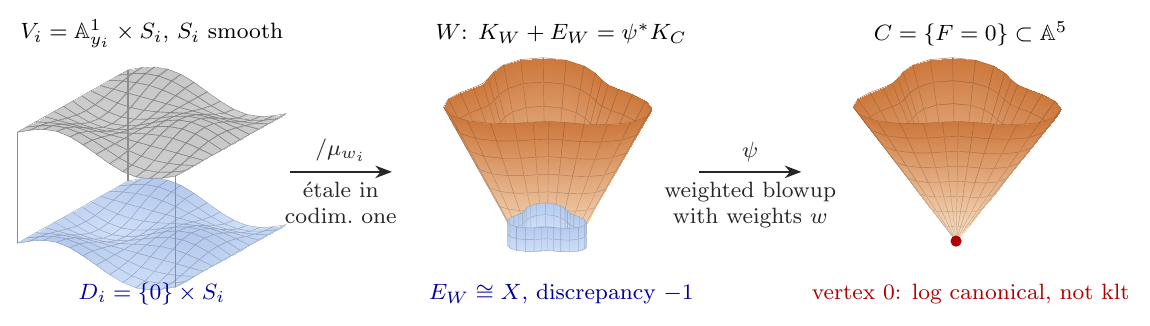
\includegraphics[width=\textwidth]{figures/fig_blowup.png}
\caption{The proof of Lemma~\ref{lem:cone}. The weighted blowup $\psi$ replaces the vertex of $C$ by $E_W\cong X$, and $K_W+E_W=\psi^*K_C$. On the chart $V_i$ the pair $(V_i,D_i)$ is a smooth variety with a smooth divisor, and $V_i\to W_i$ is a quotient by $\mu_{w_i}$ that is \'etale in codimension one.}
\label{fig:blowup}
\end{figure}

\begin{proposition}\label{prop:loc}
Let $Y=C/G$ and let $P\in Y$ be the image of $0$. Then $P\in Y$ is a four-dimensional log canonical singularity that is not klt and has index $1389$. In particular, $1389\in\Il$.
\end{proposition}

\begin{proof}
By Lemma~\ref{lem:g}(3), the fixed locus of $g^k$ on $C$ for $0<k<1389$ lies in the curve $\{x_0=x_1=x_2=0,\ x_3^3+x_4^2=0\}$. So $p\colon C\to Y$ is \'etale in codimension one, $K_C=p^*K_Y$, and $Y$ is log canonical and not klt by Lemma~\ref{lem:cone} and \cite[5.20]{KM}.

For $m\geq1$, the sections of $\mathcal O_Y(mK_Y)$ near $P$ are the $G$-invariant sections of $\omega_C^{\otimes m}$, that is, $f\sigma^m$ with $g^*f=\det(g)^{-m}f$. If $1389\mid m$, then $\sigma^m$ is invariant and generates. Conversely, if $mK_Y$ is Cartier at $P$ with generator $f\sigma^m$, then $f(0)\neq0$, and $g(0)=0$ gives $f(0)=\det(g)^{-m}f(0)$, so $1389\mid m$ by Lemma~\ref{lem:g}(2).
\end{proof}

\section{Weighted projective spaces of Fano index 1389}\label{sec:wps}

For $a=(a_0,\dots,a_4)\in\Z_{>0}^5$ with $q=\sum a_i$ and $k\in\Z$, put
\[
\age_a(k)=\sum_{i=0}^4\Big\{\frac{ka_i}{q}\Big\}=k-\sum_{i=0}^4\Big\lfloor\frac{ka_i}{q}\Big\rfloor.
\]
By Kasprzyk's criterion \cite[Proposition~2.5]{Kas}, a well-formed $\PP(a)$ has canonical singularities if and only if $\age_a(k)\in\{1,2,3\}$ for every $k\in\{2,\dots,q-2\}$.

\begin{lemma}\label{lem:witness}
Let $a\in\Z_{>0}^5$, $q=\sum a_i$, $k\in\Z$, and let $r_i\in\{0,\dots,q-1\}$ be the residue of $ka_i$ modulo $q$. If $r_i\geq1$ for $i=1,2,3,4$ and $r_1+r_2+r_3+r_4\leq q-1$, then $\age_a(q-k)=4$.
\end{lemma}

\begin{proof}
Since $\sum ka_i=kq$, we have $r_0\equiv-(r_1+\dots+r_4)\pmod q$, and $1\leq r_1+\dots+r_4\leq q-1$ gives $r_0=q-(r_1+\dots+r_4)\geq1$. All five residues are positive, so $\{(q-k)a_i/q\}=1-r_i/q$ and $\age_a(q-k)=5-\sum r_i/q=4$.
\end{proof}

\begin{proposition}\label{prop:cert}
Let $q=1389$. For all integers $1\leq a_4\leq a_3\leq a_2\leq a_1$ with $2a_1+a_2+a_3+a_4\leq q$ there is $k\in\{2,\dots,q-2\}$ such that the residues $r_i$ of $ka_i$ modulo $q$ satisfy $r_1,\dots,r_4\geq1$ and $r_1+r_2+r_3+r_4\leq q-1$.
\end{proposition}

\begin{proof}
The proof is a finite verification, carried out in the Lean kernel (Section~\ref{sec:lean}). For $t=(t_1,\dots,t_4)$ with $t_4\leq t_3\leq t_2\leq t_1$ let $x_i=1+8t_i$ and let $Q_t$ be the box $\prod_i\{x_i,\dots,x_i+7\}$. Every admissible $(a_1,\dots,a_4)$ lies in $Q_t$ for $t_i=\lfloor(a_i-1)/8\rfloor$, and then $2x_1+x_2+x_3+x_4\leq q$. There are $368{,}253$ such $t$. For each of them the certificate lists values of $k$, $2{,}624{,}293$ in all and at most $70$ per box; one value suffices for $231{,}139$ boxes. The condition on $k$ is equivalent to
\begin{equation}\label{eq:test}
\sum_{i=1}^4\big(((ka_i+q-1)\bmod q)+1\big)\leq q-1,
\end{equation}
because $((ka+q-1)\bmod q)+1$ equals the residue of $ka$ when that residue is positive and equals $q$ otherwise. Write $a_i=x_i+\delta_i$ with $0\leq\delta_i\leq7$ and $c_i=(kx_i+q-1)\bmod q$. Then $(ka_i+q-1)\bmod q=c_i+k\delta_i-q\lfloor(c_i+k\delta_i)/q\rfloor$ and
\[
\Big\lfloor\frac{c_i+k\delta_i}{q}\Big\rfloor=\#\Big\{j\geq1:\ \delta_i\geq\Big\lceil\frac{jq-c_i}{k}\Big\rceil\Big\},
\]
a sum of at most $\lfloor(c_i+7k)/q\rfloor$ indicator functions of $\delta_i$. The checker stores the $8^4$ points of a box in $17$-bit fields of one natural number and evaluates \eqref{eq:test}, the order conditions and the linear condition for all of them by additions, multiplications by integers, shifts and bitwise conjunctions; a box passes when every admissible point satisfies \eqref{eq:test} for some listed $k$. The soundness of the checker, namely that a passing box has this property, is proved in Lean, and the kernel evaluates the checker on all boxes.
\end{proof}

\begin{figure}[ht]
\centering
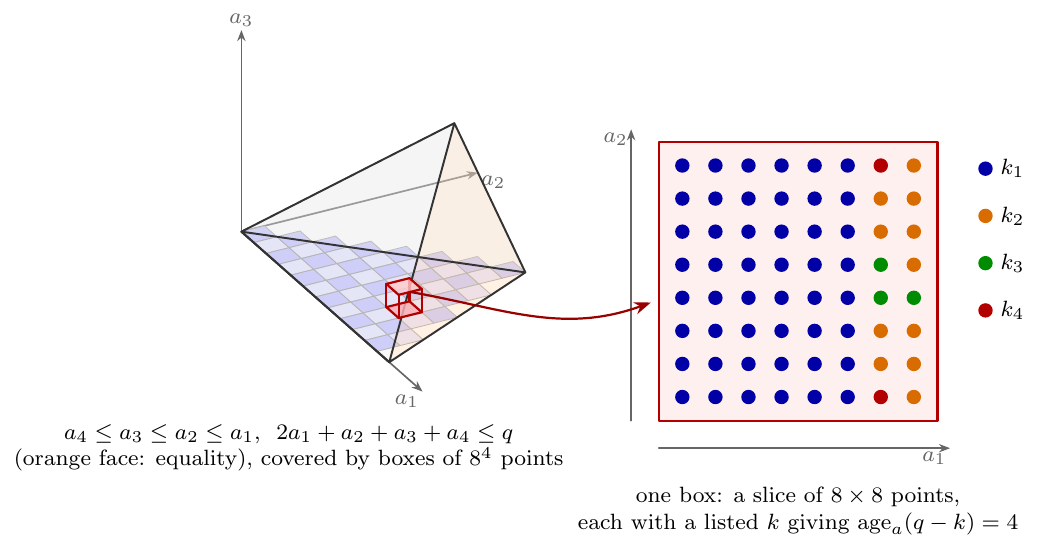
\includegraphics[width=\textwidth]{figures/fig_boxes.png}
\caption{The certificate of Proposition~\ref{prop:cert}. The sorted weights with $2a_1+a_2+a_3+a_4\leq q$ are covered by boxes of $8^4$ points (drawn in the coordinates $a_1,a_2,a_3$). For each box the certificate lists values of $k$; every point of the box is served by one of them. The right panel shows the points of one slice of one box, coloured by the listed value that serves them.}
\label{fig:boxes}
\end{figure}

\begin{theorem}\label{thm:wps}
Every $a\in\Z_{>0}^5$ with $\sum a_i=1389$ has $\age_a(k)=4$ for some $k\in\{2,\dots,1387\}$. Hence no well-formed weighted projective space $\PP(a_0,\dots,a_4)$ of Fano index $1389$ has canonical singularities, and $1389\notin\Iw$.
\end{theorem}

\begin{proof}
Order the weights so that $a_0\geq a_1\geq\dots\geq a_4$. Then $2a_1+a_2+a_3+a_4\leq a_0+\dots+a_4=1389$. Proposition~\ref{prop:cert} gives $k\in\{2,\dots,1387\}$, and Lemma~\ref{lem:witness} gives $\age_a(1389-k)=4$ with $1389-k\in\{2,\dots,1387\}$. Kasprzyk's criterion excludes canonical singularities, and $1389>4$.
\end{proof}

\begin{proof}[Proof of Theorem~\textup{\ref{thm:main}}]
Combine Propositions~\ref{prop:term} and~\ref{prop:loc} with Theorem~\ref{thm:wps}.
\end{proof}

\begin{remark}
Since $\varphi(1389)=924\leq984$, the number $1389$ lies in the set $\{m:\varphi(m)\leq984\}$ that contains $\Iw$ by \cite[Theorem~4.4]{Liu}; it is one of the elements of the set $\mathrm J_4$ of \cite[Section~4]{Liu}. Theorem~\ref{thm:wps} agrees with the list \cite{LiuData}. The neighbouring index $1383$ lies in $\Iw$: $\PP(674,461,195,35,18)$ is well formed and passes Kasprzyk's criterion.
\end{remark}

\section{Formal verification}\label{sec:lean}

The finite and algebraic parts of the proof are formalized in Lean~4 with its mathematical library \cite{Lean,Mathlib}. In the formalization the set $\Iw$ is defined as the union of $\{1,2,3,4\}$ with the sums $\sum a_i$ over the well-formed $a\in\Z_{>0}^5$ that satisfy Kasprzyk's criterion. The formal statements are Lemma~\ref{lem:F}, Lemma~\ref{lem:g}, Proposition~\ref{prop:cert}, the first part of Theorem~\ref{thm:wps}, and the statement $1389\notin\Iw$. The kernel checks every proof, and each of these theorems depends only on the axioms of propositional extensionality, choice and quotient soundness.

The certificate of Proposition~\ref{prop:cert} is split into $4{,}022$ statements, each asserting that the checker accepts one list of boxes. Each statement is closed by evaluating the checker in the kernel, so no compiled code is trusted; checking all of them takes about $15$ minutes on four cores. The steps that rest on the literature, namely Kasprzyk's criterion, the results of \cite{IF} and \cite{ETW}, and the singularity theory of Sections~\ref{sec:x}--\ref{sec:loc}, are proved in the text and not formalized, since the library does not yet contain weighted projective spaces or discrepancies.

Independently of the formalization, programs in C, C++, Julia and Python enumerate all $1{,}301{,}769{,}806$ partitions of $1389$ into five parts, test Kasprzyk's criterion on the $874{,}763{,}737$ well-formed ones, and find no canonical one. The same enumeration for $q=1383$ finds $\PP(674,461,195,35,18)$.

\section*{Acknowledgements}
The authors used the generative AI tool Claude (Anthropic), through Claude Code, to assist with the proofs, the Lean formalization, the computations and the preparation of this article. The authors reviewed and edited the content and take full responsibility for it.

\section*{Competing interests}
None.

\section*{Funding}
None.

\section*{Data availability}
\begingroup\raggedright
\ifanon
The computations and the Lean formalization were carried out by the authors with the help of AI assistance (Claude, Anthropic). The Lean formalization, the certificate generator and the search programs are supplied with the submission.\par
\else
Deep Bhattacharjee computed the Lean formalization and the Julia, C, C++, shell and Python computations with the help of AI assistance (Claude, Anthropic). The Lean formalization of the finite and algebraic parts of the proof, together with the certificate generator and the search programs, is archived at Zenodo \cite{archive}, doi:\href{https://doi.org/\zenodoID}{\zenodoID}. The paper is available at \url{\preprintURL}.\par
\fi
\endgroup

\begin{thebibliography}{99}
\raggedright

\ifanon\else
\bibitem{archive}
D.~Bhattacharjee and U.~Bhattacharya, \emph{A counterexample to Liu's conjecture on Fano indices in dimension four: Lean formalization and programs}, Zenodo, 2026, doi:\href{https://doi.org/\zenodoID}{\zenodoID}.
\fi

\bibitem{Mathlib}
The mathlib Community, \emph{The Lean mathematical library}, in: Proceedings of the 9th ACM SIGPLAN International Conference on Certified Programs and Proofs (CPP 2020), ACM, 2020, pp.~367--381, doi:\href{https://doi.org/10.1145/3372885.3373824}{10.1145/3372885.3373824}.

\bibitem{ETW}
L.~Esser, B.~Totaro and C.~Wang, \emph{Calabi--Yau varieties of large index}, Algebr. Geom., to appear; arXiv:2209.04597.

\bibitem{IF}
A.~R.~Iano-Fletcher, \emph{Working with weighted complete intersections}, in: Explicit birational geometry of 3-folds, London Math. Soc. Lecture Note Ser. 281, Cambridge Univ. Press, Cambridge, 2000, pp.~101--174, doi:\href{https://doi.org/10.1017/CBO9780511758942.005}{10.1017/CBO9780511758942.005}.

\bibitem{Kas}
A.~M.~Kasprzyk, \emph{Classifying terminal weighted projective space}, arXiv:1304.3029.

\bibitem{KM}
J.~Koll\'ar and S.~Mori, \emph{Birational geometry of algebraic varieties}, Cambridge Tracts in Math. 134, Cambridge Univ. Press, Cambridge, 1998, doi:\href{https://doi.org/10.1017/CBO9780511662560}{10.1017/CBO9780511662560}.

\bibitem{Liu}
H.~Liu, \emph{On Fano indices of weighted projective spaces}, arXiv:2608.03434v3, 2026.

\bibitem{LiuData}
H.~Liu, \emph{Fano indices of four-dimensional canonical weighted projective spaces} (data and code), Zenodo, doi:\href{https://doi.org/10.5281/zenodo.21806548}{10.5281/zenodo.21806548}.

\bibitem{Lean}
L.~de~Moura and S.~Ullrich, \emph{The Lean~4 theorem prover and programming language}, in: Automated Deduction -- CADE 28, Lecture Notes in Comput. Sci. 12699, Springer, 2021, pp.~625--635, doi:\href{https://doi.org/10.1007/978-3-030-79876-5_37}{10.1007/978-3-030-79876-5\_37}.

\end{thebibliography}

\end{document}
"  for the anonymized
% version required by the double-anonymous review of the journal.
\newif\ifanon
\ifdefined\anonymous\anontrue\fi

\newtheorem{theorem}{Theorem}[section]
\newtheorem{lemma}[theorem]{Lemma}
\newtheorem{proposition}[theorem]{Proposition}
\newtheorem{conjecture}[theorem]{Conjecture}
\theoremstyle{remark}
\newtheorem{remark}[theorem]{Remark}

\DeclareMathOperator{\age}{age}
\newcommand{\Iw}{\mathrm{I}_{4,\mathrm{wps}}}
\newcommand{\It}{\mathrm{I}_{4,\mathrm{term}}}
\newcommand{\Il}{\mathrm{I}_{4,\mathrm{loc}}}
\newcommand{\C}{\mathbb{C}}
\newcommand{\Z}{\mathbb{Z}}
\newcommand{\PP}{\mathbb{P}}
\newcommand{\A}{\mathbb{A}}
\newcommand{\zenodoID}{10.5281/zenodo.23387505}
\newcommand{\preprintURL}{https://github.com/creelie/fuzzy-guacamole/blob/main/preprintLiuFanoIndexConjecture/LiuFanoIndexConjecture.pdf}

\begin{document}

\title[Liu's conjecture on Fano indices]{A counterexample to Liu's conjecture on Fano indices in dimension four}

\ifanon\else
\author{Deep Bhattacharjee}
\address{Formerly, Electro-Gravitational Space Propulsion Laboratory (EGSPL),\newline Bhubaneswar, Odisha 751030, India}
\email{itsdeep@live.com}
\email{d.bhattacharjee@erl-forschung.de}
\author{Ushashi Bhattacharya}
\address{Formerly, National Taiwan University, Taipei 106319, Taiwan}
\email{rai.bhattacharya.in@gmail.com}
\thanks{Corresponding author: Deep Bhattacharjee. ORCID iDs: Deep Bhattacharjee 0000-0003-0466-750X; Ushashi Bhattacharya 0009-0002-2254-3914.}
\fi

\subjclass[2020]{Primary 14J32; Secondary 14B05, 14J45, 14M25}
\keywords{Fano index, weighted projective space, Calabi--Yau variety, log canonical singularity, index}

\begin{abstract}
We prove that Liu's conjecture on Fano indices fails in dimension four: $1389$ is the index of a terminal Calabi--Yau fourfold and of a four-dimensional log canonical singularity, but it is not the Fano index of any canonical weighted projective space of dimension four.
\end{abstract}

\maketitle

\section{Introduction}

We work over $\C$. For a well-formed weighted projective space $\PP(a_0,\dots,a_n)$ with canonical singularities, the Fano index is $q=a_0+\dots+a_n$. The \emph{index} of a Calabi--Yau variety $S$ (a normal projective variety with $K_S\sim_{\mathbb Q}0$) is the least $m\geq1$ with $mK_S\sim0$, and the index of a log canonical singularity $P\in Y$ is the least $m\geq1$ such that $mK_Y$ is Cartier at $P$. Following \cite[Definition~4.1]{Liu}, let
\begin{itemize}
\item $\mathrm{I}_{n,\mathrm{wps}}$ be the set of Fano indices of $n$-dimensional well-formed weighted projective spaces with canonical singularities, together with $\{1,\dots,n\}$;
\item $\mathrm{I}_{n,\mathrm{term}}$ be the set of indices of $n$-dimensional terminal Calabi--Yau varieties;
\item $\mathrm{I}_{n,\mathrm{loc}}$ be the set of indices of $n$-dimensional log canonical singularities.
\end{itemize}

\begin{conjecture}[{\cite[Conjecture~4.2]{Liu}}]\label{conj:liu}
$\mathrm{I}_{n,\mathrm{wps}}=\mathrm{I}_{n,\mathrm{term}}=\mathrm{I}_{n,\mathrm{loc}}$ for every $n\geq2$.
\end{conjecture}

Liu proves the conjecture for $n\leq3$ \cite[Proposition~4.3]{Liu} and computes $\Iw$ by an exhaustive search \cite[Theorem~4.4]{Liu}, \cite{LiuData}.

\begin{theorem}\label{thm:main}
$1389\in\It\cap\Il$ and $1389\notin\Iw$. In particular, Conjecture~\ref{conj:liu} fails for $n=4$.
\end{theorem}

The two memberships come from a symmetry of order $1389$ of one Calabi--Yau threefold, the hypersurface $X_{78}$ of $\PP(1,1,11,26,39)$ (Sections~\ref{sec:x}--\ref{sec:loc}). The non-membership is a finite statement about the $1{,}301{,}769{,}806$ partitions of $1389$ into five parts (Section~\ref{sec:wps}). It is proved in the Lean~4 kernel from a certificate of witnesses, together with the polynomial identities of Section~\ref{sec:x} (Section~\ref{sec:lean}). Figure~\ref{fig:roadmap} shows the plan of the proof.

\begin{figure}[ht]
\centering
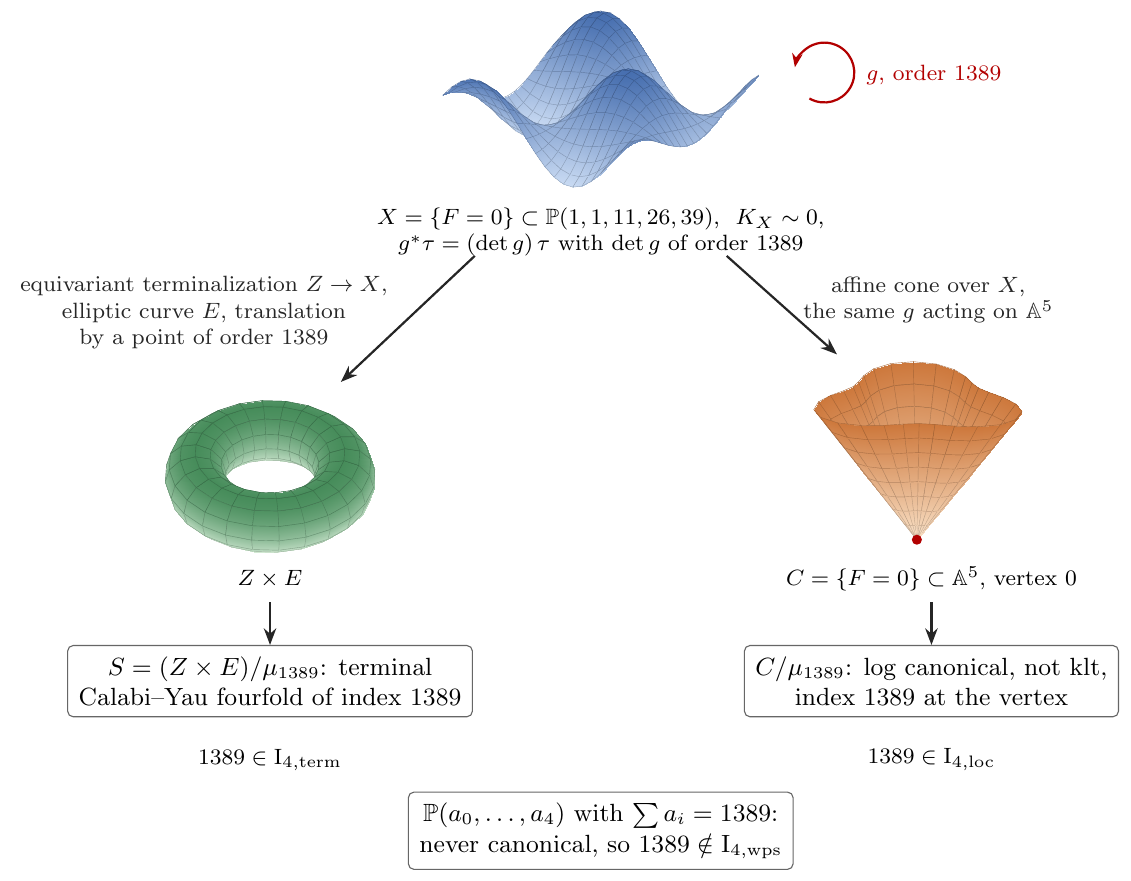
\includegraphics[width=\textwidth]{figures/fig_roadmap.png}
\caption{The plan of the proof. One symmetry $g$ of order $1389$ of the threefold $X$ gives a terminal Calabi--Yau fourfold of index $1389$ (Section~\ref{sec:term}) and a log canonical singularity of index $1389$ (Section~\ref{sec:loc}); no canonical weighted projective fourspace has Fano index $1389$ (Section~\ref{sec:wps}).}
\label{fig:roadmap}
\end{figure}

\begin{remark}\label{rem:literal}
Read literally, $\Il$ contains every positive integer: for $m\geq2$ the group $\mu_m$ acting on $\C^4$ with weights $(1,1,1,m-2)$ is free in codimension one, so $\C^4/\mu_m$ is klt, and $dx_1\wedge\dots\wedge dx_4$ has weight $m+1\equiv1\pmod m$, so its index is $m$ (by the argument in the proof of Proposition~\ref{prop:loc}). Since $3487\notin\Iw$ by \cite[Theorem~4.4]{Liu}, the literal reading fails at once, and the intended reading of $\mathrm{I}_{n,\mathrm{loc}}$ concerns log canonical singularities that are not klt. The singularity of Proposition~\ref{prop:loc} is log canonical and not klt, so Theorem~\ref{thm:main} holds for both readings.
\end{remark}

\section{The threefold}\label{sec:x}

Let $w=(w_0,\dots,w_4)=(1,1,11,26,39)$ and
\[
F=x_0^{77}x_1+x_1^{67}x_2+x_2^{7}x_0+x_3^3+x_4^2\in\C[x_0,\dots,x_4].
\]

\begin{lemma}\label{lem:F}
\begin{enumerate}
\item $F$ is quasi-homogeneous of degree $78=w_0+\dots+w_4$ for the weights $w$.
\item Any three of the $w_i$ are coprime.
\item The partial derivatives of $F$ have no common zero in $\C^5$ other than $0$.
\end{enumerate}
\end{lemma}

\begin{proof}
(1) and (2) are direct. For (3), let $x$ be a common zero; then $x_3=x_4=0$. With $\partial_i=\partial F/\partial x_i$,
\[
x_0\partial_0-77\,x_1\partial_1+5159\,x_2\partial_2=36114\,x_2^7x_0,
\]
since $x_0\partial_0=77x_0^{77}x_1+x_2^7x_0$, $x_1\partial_1=x_0^{77}x_1+67x_1^{67}x_2$ and $x_2\partial_2=x_1^{67}x_2+7x_2^7x_0$. Hence $x_2^7x_0=0$. If $x_2=0$, then $\partial_1=x_0^{77}$ and $\partial_2=x_1^{67}+7x_2^6x_0$ give $x_0=x_1=0$. If $x_0=0$, then $\partial_0=x_2^7$ gives $x_2=0$ and $\partial_2$ gives $x_1=0$.
\end{proof}

Let $C=\{F=0\}\subset\A^5$ and $X=\{F=0\}\subset\PP=\PP(1,1,11,26,39)$. By Lemma~\ref{lem:F}, $X$ is a quasi-smooth hypersurface of degree $78$; $\PP$ and $X$ are well formed \cite[6.10]{IF}. Hence $X$ has cyclic quotient singularities and $\omega_X\cong\mathcal O_X(78-\sum w_i)=\mathcal O_X$ \cite[6.14]{IF}. Quotient singularities are klt \cite[5.20]{KM}, and the discrepancies of a klt variety with Cartier canonical divisor are integers, so $X$ is a canonical Calabi--Yau threefold with $K_X\sim0$.

Fix a primitive $1389$th root of unity $\zeta$ and put $g=\operatorname{diag}(\zeta,\zeta^{1312},\zeta^{992},1,1)$.

\begin{lemma}\label{lem:g}
\begin{enumerate}
\item $F(gx)=F(x)$.
\item $\det g=\zeta^{2305}$ is a primitive $1389$th root of unity.
\item For $0<k<1389$, every fixed point $x\in\C^5$ of $g^k$ has $x_0=x_1=x_2=0$.
\end{enumerate}
\end{lemma}

\begin{proof}
(1) The monomials $x_0^{77}x_1$, $x_1^{67}x_2$ and $x_2^7x_0$ acquire the factors
\[
\zeta^{77+1312}=\zeta^{1389},\qquad\zeta^{67\cdot1312+992}=\zeta^{64\cdot1389},\qquad\zeta^{7\cdot992+1}=\zeta^{5\cdot1389}.
\] (2) $1389=3\cdot463$ and $2305=5\cdot461$ are coprime. (3) The integers $1$, $1312=2^5\cdot41$ and $992=2^5\cdot31$ are prime to $1389$, so $\zeta^k$, $\zeta^{1312k}$ and $\zeta^{992k}$ differ from $1$.
\end{proof}

The matrix $g$ commutes with the $\C^*$-action $t\cdot x=(t^{w_0}x_0,\dots,t^{w_4}x_4)$, so $G=\langle g\rangle\cong\mu_{1389}$ acts on $C$, on $\PP$ and on $X$. Let $\sigma$ be the Poincar\'e residue of $dx_0\wedge\dots\wedge dx_4/F$ along $C$; it generates $\omega_C$, and $g^*\sigma=\det(g)\,\sigma$ by Lemma~\ref{lem:g}(1).

\begin{lemma}\label{lem:omega}
$H^0(X,\omega_X)$ is spanned by a form $\tau$ with $g^*\tau=\det(g)\,\tau$.
\end{lemma}

\begin{proof}
Let $\xi=\sum w_ix_i\,\partial/\partial x_i$ and let $\rho\colon C\setminus\{0\}\to X$ be the quotient map. The $3$-form $\iota_\xi\sigma$ is $\C^*$-invariant, since $\sigma$ has weight $\sum w_i-78=0$, and $\iota_\xi\iota_\xi\sigma=0$. Let $X^\circ\subset X$ be the open set over which $\rho$ is a principal $\C^*$-bundle; its complement has codimension at least $2$ because $X$ is well formed. On $X^\circ$ there is a nowhere vanishing $3$-form $\tau$ with $\rho^*\tau=\iota_\xi\sigma$. As $\omega_X$ is reflexive, $\tau$ is a nowhere vanishing section of $\omega_X\cong\mathcal O_X$, so it spans $H^0(X,\omega_X)$. Since $g$ commutes with $\xi$ and with $\rho$, $g^*\tau=\det(g)\,\tau$.
\end{proof}

\section{A terminal Calabi--Yau fourfold of index 1389}\label{sec:term}

\begin{proposition}\label{prop:term}
$1389\in\It$.
\end{proposition}

\begin{proof}
By \cite[Proposition~2.2]{ETW} there is a $G$-equivariant projective birational morphism $\pi\colon Z\to X$ with $Z$ terminal and $K_Z=\pi^*K_X$. Then $\pi^*\tau$ is a nowhere vanishing section of $\omega_Z$, and $g^*\pi^*\tau=\det(g)\,\pi^*\tau$ by Lemma~\ref{lem:omega}. Let $E$ be an elliptic curve with a point $p$ of order $1389$, and let $G$ act on $Z\times E$ by $g(z,e)=(gz,e+p)$. The action is free, so $S=(Z\times E)/G$ is a terminal projective fourfold and $Z\times E\to S$ is \'etale. With $\eta$ a translation-invariant $1$-form on $E$, the form $\pi^*\tau\wedge\eta$ spans $H^0(Z\times E,\omega_{Z\times E})$ and $g$ multiplies it by $\det(g)$. For $m\geq1$, the sections of $\mathcal O_S(mK_S)$ are the $G$-invariant sections of $\omega_{Z\times E}^{\otimes m}$, so $H^0(S,\mathcal O_S(mK_S))\neq0$ if and only if $\det(g)^m=1$, that is, $1389\mid m$. As $K_S$ is numerically trivial, a nonzero section of $\mathcal O_S(mK_S)$ has no zeros, so $mK_S\sim0$ exactly when $1389\mid m$. This is the argument of \cite[Corollary~4.1]{ETW}. Hence $S$ is a terminal Calabi--Yau fourfold of index $1389$.
\end{proof}

\section{A log canonical singularity of index 1389}\label{sec:loc}

\begin{lemma}\label{lem:cone}
$C$ is normal and Gorenstein, log canonical, and not klt.
\end{lemma}

\begin{proof}
By Lemma~\ref{lem:F}(3), $C$ is a hypersurface whose only singular point is $0$, so $C$ is Gorenstein and, by Serre's criterion, normal; its local ring at $0$ is a domain, so $C$ is irreducible and no coordinate $x_j$ divides $F$.

Let $B\to\A^5$ be the weighted blow-up of $0$ with weights $w$. It is covered by the charts $U_i=\A^5/\mu_{w_i}$, where $\varphi_i\colon\A^5_y\to\A^5_x$ is $x_i=y_i^{w_i}$, $x_j=y_jy_i^{w_j}$ ($j\neq i$), and $\varepsilon\in\mu_{w_i}$ acts by $y_i\mapsto\varepsilon y_i$, $y_j\mapsto\varepsilon^{-w_j}y_j$. Quasi-homogeneity gives $F\circ\varphi_i=y_i^{78}F_i$, where $F_i$ is $F$ with $x_i$ replaced by $1$ and $x_j$ by $y_j$; it does not involve $y_i$. Let $S_i=\{F_i=0\}$ in the coordinates $y_j$, $j\neq i$. If $F_i$ and its derivatives vanish at $u$ (with $u_i=1$), the Euler identity $78F=\sum w_jx_j\partial_jF$ gives $\partial_iF(u)=0$, contradicting Lemma~\ref{lem:F}(3); so $S_i$ is smooth. The strict transform $W$ of $C$ is covered by $W_i=V_i/\mu_{w_i}$ with $V_i=\A^1_{y_i}\times S_i$, and the exceptional divisor $E_W=W\cap\pi^{-1}(0)$ is covered by $D_i/\mu_{w_i}$ with $D_i=\{0\}\times S_i$.

The action of $\mu_{w_i}$ on $V_i$ is free in codimension one. A non-identity $\varepsilon$ fixes no point with $y_i\neq0$. Its fixed points in $D_i$ satisfy $y_j=0$ for some $j\neq i$ with $\varepsilon^{w_j}\neq1$, which exists because the $w_j$ with $j\neq i$ are coprime; and $\{y_j=0\}$ contains no component of $S_i$ because $x_j\nmid F$. Hence $q_i\colon V_i\to W_i$ is \'etale in codimension one, $q_i^*K_{W_i}=K_{V_i}$ and $q_i^*E_W=D_i$. The pair $(V_i,D_i)$ is a smooth variety with a smooth divisor, hence log canonical, so $(W,E_W)$ is log canonical by \cite[5.20]{KM}.

The Jacobian of $\varphi_i$ is $w_iy_i^{\sum w_j-1}$, so
\[
\varphi_i^*(dx/F)=w_iy_i^{\sum w_j-1-78}\,dy/F_i=w_iy_i^{-1}\,dy/F_i,
\]
and the pullback of $\sigma$ to $V_i$ is $w_iy_i^{-1}$ times a generator of $\omega_{V_i}$. Thus the pullback of $\sigma$ to $W$ is a rational section of $\omega_W$ with divisor $-E_W$, that is, $K_W+E_W=\psi^*K_C$ for $\psi\colon W\to C$. By \cite[Lemma~2.30]{KM}, every divisor over $C$ has the same discrepancy for $C$ as for $(W,E_W)$. So $C$ is log canonical, and $E_W$ has discrepancy $-1$, so $C$ is not klt.
\end{proof}

\begin{figure}[ht]
\centering
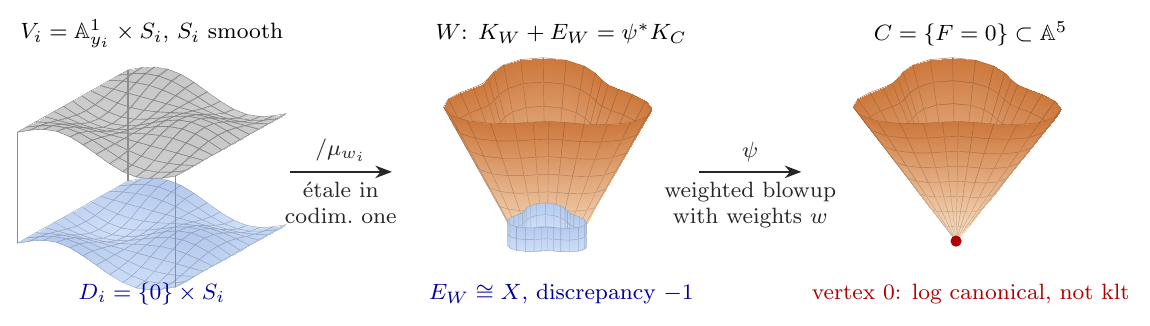
\includegraphics[width=\textwidth]{figures/fig_blowup.png}
\caption{The proof of Lemma~\ref{lem:cone}. The weighted blowup $\psi$ replaces the vertex of $C$ by $E_W\cong X$, and $K_W+E_W=\psi^*K_C$. On the chart $V_i$ the pair $(V_i,D_i)$ is a smooth variety with a smooth divisor, and $V_i\to W_i$ is a quotient by $\mu_{w_i}$ that is \'etale in codimension one.}
\label{fig:blowup}
\end{figure}

\begin{proposition}\label{prop:loc}
Let $Y=C/G$ and let $P\in Y$ be the image of $0$. Then $P\in Y$ is a four-dimensional log canonical singularity that is not klt and has index $1389$. In particular, $1389\in\Il$.
\end{proposition}

\begin{proof}
By Lemma~\ref{lem:g}(3), the fixed locus of $g^k$ on $C$ for $0<k<1389$ lies in the curve $\{x_0=x_1=x_2=0,\ x_3^3+x_4^2=0\}$. So $p\colon C\to Y$ is \'etale in codimension one, $K_C=p^*K_Y$, and $Y$ is log canonical and not klt by Lemma~\ref{lem:cone} and \cite[5.20]{KM}.

For $m\geq1$, the sections of $\mathcal O_Y(mK_Y)$ near $P$ are the $G$-invariant sections of $\omega_C^{\otimes m}$, that is, $f\sigma^m$ with $g^*f=\det(g)^{-m}f$. If $1389\mid m$, then $\sigma^m$ is invariant and generates. Conversely, if $mK_Y$ is Cartier at $P$ with generator $f\sigma^m$, then $f(0)\neq0$, and $g(0)=0$ gives $f(0)=\det(g)^{-m}f(0)$, so $1389\mid m$ by Lemma~\ref{lem:g}(2).
\end{proof}

\section{Weighted projective spaces of Fano index 1389}\label{sec:wps}

For $a=(a_0,\dots,a_4)\in\Z_{>0}^5$ with $q=\sum a_i$ and $k\in\Z$, put
\[
\age_a(k)=\sum_{i=0}^4\Big\{\frac{ka_i}{q}\Big\}=k-\sum_{i=0}^4\Big\lfloor\frac{ka_i}{q}\Big\rfloor.
\]
By Kasprzyk's criterion \cite[Proposition~2.5]{Kas}, a well-formed $\PP(a)$ has canonical singularities if and only if $\age_a(k)\in\{1,2,3\}$ for every $k\in\{2,\dots,q-2\}$.

\begin{lemma}\label{lem:witness}
Let $a\in\Z_{>0}^5$, $q=\sum a_i$, $k\in\Z$, and let $r_i\in\{0,\dots,q-1\}$ be the residue of $ka_i$ modulo $q$. If $r_i\geq1$ for $i=1,2,3,4$ and $r_1+r_2+r_3+r_4\leq q-1$, then $\age_a(q-k)=4$.
\end{lemma}

\begin{proof}
Since $\sum ka_i=kq$, we have $r_0\equiv-(r_1+\dots+r_4)\pmod q$, and $1\leq r_1+\dots+r_4\leq q-1$ gives $r_0=q-(r_1+\dots+r_4)\geq1$. All five residues are positive, so $\{(q-k)a_i/q\}=1-r_i/q$ and $\age_a(q-k)=5-\sum r_i/q=4$.
\end{proof}

\begin{proposition}\label{prop:cert}
Let $q=1389$. For all integers $1\leq a_4\leq a_3\leq a_2\leq a_1$ with $2a_1+a_2+a_3+a_4\leq q$ there is $k\in\{2,\dots,q-2\}$ such that the residues $r_i$ of $ka_i$ modulo $q$ satisfy $r_1,\dots,r_4\geq1$ and $r_1+r_2+r_3+r_4\leq q-1$.
\end{proposition}

\begin{proof}
The proof is a finite verification, carried out in the Lean kernel (Section~\ref{sec:lean}). For $t=(t_1,\dots,t_4)$ with $t_4\leq t_3\leq t_2\leq t_1$ let $x_i=1+8t_i$ and let $Q_t$ be the box $\prod_i\{x_i,\dots,x_i+7\}$. Every admissible $(a_1,\dots,a_4)$ lies in $Q_t$ for $t_i=\lfloor(a_i-1)/8\rfloor$, and then $2x_1+x_2+x_3+x_4\leq q$. There are $368{,}253$ such $t$. For each of them the certificate lists values of $k$, $2{,}624{,}293$ in all and at most $70$ per box; one value suffices for $231{,}139$ boxes. The condition on $k$ is equivalent to
\begin{equation}\label{eq:test}
\sum_{i=1}^4\big(((ka_i+q-1)\bmod q)+1\big)\leq q-1,
\end{equation}
because $((ka+q-1)\bmod q)+1$ equals the residue of $ka$ when that residue is positive and equals $q$ otherwise. Write $a_i=x_i+\delta_i$ with $0\leq\delta_i\leq7$ and $c_i=(kx_i+q-1)\bmod q$. Then $(ka_i+q-1)\bmod q=c_i+k\delta_i-q\lfloor(c_i+k\delta_i)/q\rfloor$ and
\[
\Big\lfloor\frac{c_i+k\delta_i}{q}\Big\rfloor=\#\Big\{j\geq1:\ \delta_i\geq\Big\lceil\frac{jq-c_i}{k}\Big\rceil\Big\},
\]
a sum of at most $\lfloor(c_i+7k)/q\rfloor$ indicator functions of $\delta_i$. The checker stores the $8^4$ points of a box in $17$-bit fields of one natural number and evaluates \eqref{eq:test}, the order conditions and the linear condition for all of them by additions, multiplications by integers, shifts and bitwise conjunctions; a box passes when every admissible point satisfies \eqref{eq:test} for some listed $k$. The soundness of the checker, namely that a passing box has this property, is proved in Lean, and the kernel evaluates the checker on all boxes.
\end{proof}

\begin{figure}[ht]
\centering
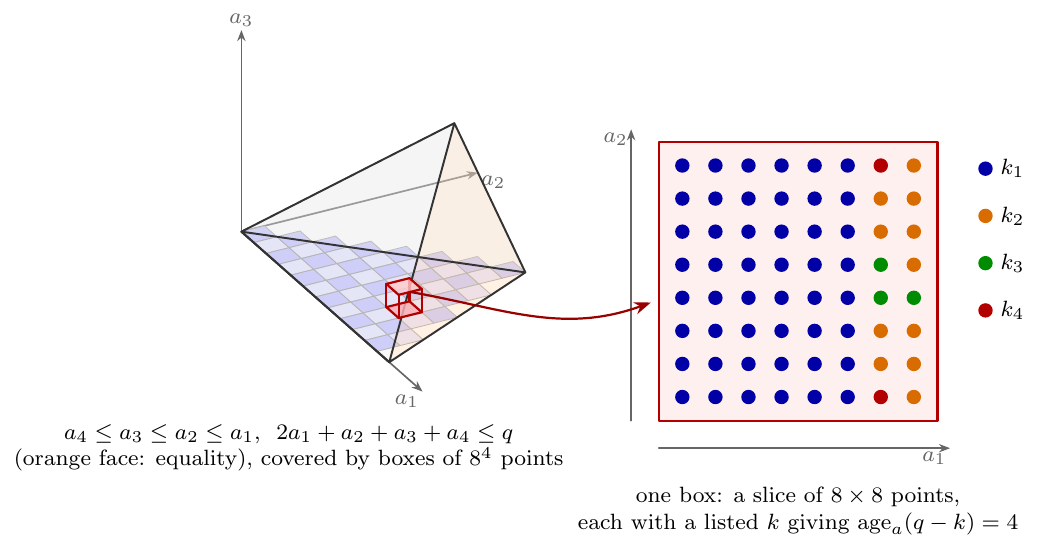
\includegraphics[width=\textwidth]{figures/fig_boxes.png}
\caption{The certificate of Proposition~\ref{prop:cert}. The sorted weights with $2a_1+a_2+a_3+a_4\leq q$ are covered by boxes of $8^4$ points (drawn in the coordinates $a_1,a_2,a_3$). For each box the certificate lists values of $k$; every point of the box is served by one of them. The right panel shows the points of one slice of one box, coloured by the listed value that serves them.}
\label{fig:boxes}
\end{figure}

\begin{theorem}\label{thm:wps}
Every $a\in\Z_{>0}^5$ with $\sum a_i=1389$ has $\age_a(k)=4$ for some $k\in\{2,\dots,1387\}$. Hence no well-formed weighted projective space $\PP(a_0,\dots,a_4)$ of Fano index $1389$ has canonical singularities, and $1389\notin\Iw$.
\end{theorem}

\begin{proof}
Order the weights so that $a_0\geq a_1\geq\dots\geq a_4$. Then $2a_1+a_2+a_3+a_4\leq a_0+\dots+a_4=1389$. Proposition~\ref{prop:cert} gives $k\in\{2,\dots,1387\}$, and Lemma~\ref{lem:witness} gives $\age_a(1389-k)=4$ with $1389-k\in\{2,\dots,1387\}$. Kasprzyk's criterion excludes canonical singularities, and $1389>4$.
\end{proof}

\begin{proof}[Proof of Theorem~\textup{\ref{thm:main}}]
Combine Propositions~\ref{prop:term} and~\ref{prop:loc} with Theorem~\ref{thm:wps}.
\end{proof}

\begin{remark}
Since $\varphi(1389)=924\leq984$, the number $1389$ lies in the set $\{m:\varphi(m)\leq984\}$ that contains $\Iw$ by \cite[Theorem~4.4]{Liu}; it is one of the elements of the set $\mathrm J_4$ of \cite[Section~4]{Liu}. Theorem~\ref{thm:wps} agrees with the list \cite{LiuData}. The neighbouring index $1383$ lies in $\Iw$: $\PP(674,461,195,35,18)$ is well formed and passes Kasprzyk's criterion.
\end{remark}

\section{Formal verification}\label{sec:lean}

The finite and algebraic parts of the proof are formalized in Lean~4 with its mathematical library \cite{Lean,Mathlib}. In the formalization the set $\Iw$ is defined as the union of $\{1,2,3,4\}$ with the sums $\sum a_i$ over the well-formed $a\in\Z_{>0}^5$ that satisfy Kasprzyk's criterion. The formal statements are Lemma~\ref{lem:F}, Lemma~\ref{lem:g}, Proposition~\ref{prop:cert}, the first part of Theorem~\ref{thm:wps}, and the statement $1389\notin\Iw$. The kernel checks every proof, and each of these theorems depends only on the axioms of propositional extensionality, choice and quotient soundness.

The certificate of Proposition~\ref{prop:cert} is split into $4{,}022$ statements, each asserting that the checker accepts one list of boxes. Each statement is closed by evaluating the checker in the kernel, so no compiled code is trusted; checking all of them takes about $15$ minutes on four cores. The steps that rest on the literature, namely Kasprzyk's criterion, the results of \cite{IF} and \cite{ETW}, and the singularity theory of Sections~\ref{sec:x}--\ref{sec:loc}, are proved in the text and not formalized, since the library does not yet contain weighted projective spaces or discrepancies.

Independently of the formalization, programs in C, C++, Julia and Python enumerate all $1{,}301{,}769{,}806$ partitions of $1389$ into five parts, test Kasprzyk's criterion on the $874{,}763{,}737$ well-formed ones, and find no canonical one. The same enumeration for $q=1383$ finds $\PP(674,461,195,35,18)$.

\section*{Acknowledgements}
The authors used the generative AI tool Claude (Anthropic), through Claude Code, to assist with the proofs, the Lean formalization, the computations and the preparation of this article. The authors reviewed and edited the content and take full responsibility for it.

\section*{Competing interests}
None.

\section*{Funding}
None.

\section*{Data availability}
\begingroup\raggedright
\ifanon
The computations and the Lean formalization were carried out by the authors with the help of AI assistance (Claude, Anthropic). The Lean formalization, the certificate generator and the search programs are supplied with the submission.\par
\else
Deep Bhattacharjee computed the Lean formalization and the Julia, C, C++, shell and Python computations with the help of AI assistance (Claude, Anthropic). The Lean formalization of the finite and algebraic parts of the proof, together with the certificate generator and the search programs, is archived at Zenodo \cite{archive}, doi:\href{https://doi.org/\zenodoID}{\zenodoID}. The paper is available at \url{\preprintURL}.\par
\fi
\endgroup

\begin{thebibliography}{99}
\raggedright

\ifanon\else
\bibitem{archive}
D.~Bhattacharjee and U.~Bhattacharya, \emph{A counterexample to Liu's conjecture on Fano indices in dimension four: Lean formalization and programs}, Zenodo, 2026, doi:\href{https://doi.org/\zenodoID}{\zenodoID}.
\fi

\bibitem{Mathlib}
The mathlib Community, \emph{The Lean mathematical library}, in: Proceedings of the 9th ACM SIGPLAN International Conference on Certified Programs and Proofs (CPP 2020), ACM, 2020, pp.~367--381, doi:\href{https://doi.org/10.1145/3372885.3373824}{10.1145/3372885.3373824}.

\bibitem{ETW}
L.~Esser, B.~Totaro and C.~Wang, \emph{Calabi--Yau varieties of large index}, Algebr. Geom., to appear; arXiv:2209.04597.

\bibitem{IF}
A.~R.~Iano-Fletcher, \emph{Working with weighted complete intersections}, in: Explicit birational geometry of 3-folds, London Math. Soc. Lecture Note Ser. 281, Cambridge Univ. Press, Cambridge, 2000, pp.~101--174, doi:\href{https://doi.org/10.1017/CBO9780511758942.005}{10.1017/CBO9780511758942.005}.

\bibitem{Kas}
A.~M.~Kasprzyk, \emph{Classifying terminal weighted projective space}, arXiv:1304.3029.

\bibitem{KM}
J.~Koll\'ar and S.~Mori, \emph{Birational geometry of algebraic varieties}, Cambridge Tracts in Math. 134, Cambridge Univ. Press, Cambridge, 1998, doi:\href{https://doi.org/10.1017/CBO9780511662560}{10.1017/CBO9780511662560}.

\bibitem{Liu}
H.~Liu, \emph{On Fano indices of weighted projective spaces}, arXiv:2608.03434v3, 2026.

\bibitem{LiuData}
H.~Liu, \emph{Fano indices of four-dimensional canonical weighted projective spaces} (data and code), Zenodo, doi:\href{https://doi.org/10.5281/zenodo.21806548}{10.5281/zenodo.21806548}.

\bibitem{Lean}
L.~de~Moura and S.~Ullrich, \emph{The Lean~4 theorem prover and programming language}, in: Automated Deduction -- CADE 28, Lecture Notes in Comput. Sci. 12699, Springer, 2021, pp.~625--635, doi:\href{https://doi.org/10.1007/978-3-030-79876-5_37}{10.1007/978-3-030-79876-5\_37}.

\end{thebibliography}

\end{document}
"  for the anonymized
% version required by the double-anonymous review of the journal.
\newif\ifanon
\ifdefined\anonymous\anontrue\fi

\newtheorem{theorem}{Theorem}[section]
\newtheorem{lemma}[theorem]{Lemma}
\newtheorem{proposition}[theorem]{Proposition}
\newtheorem{conjecture}[theorem]{Conjecture}
\theoremstyle{remark}
\newtheorem{remark}[theorem]{Remark}

\DeclareMathOperator{\age}{age}
\newcommand{\Iw}{\mathrm{I}_{4,\mathrm{wps}}}
\newcommand{\It}{\mathrm{I}_{4,\mathrm{term}}}
\newcommand{\Il}{\mathrm{I}_{4,\mathrm{loc}}}
\newcommand{\C}{\mathbb{C}}
\newcommand{\Z}{\mathbb{Z}}
\newcommand{\PP}{\mathbb{P}}
\newcommand{\A}{\mathbb{A}}
\newcommand{\zenodoID}{10.5281/zenodo.23387505}
\newcommand{\preprintURL}{https://github.com/creelie/fuzzy-guacamole/blob/main/preprintLiuFanoIndexConjecture/LiuFanoIndexConjecture.pdf}

\begin{document}

\title[Liu's conjecture on Fano indices]{A counterexample to Liu's conjecture on Fano indices in dimension four}

\ifanon\else
\author{Deep Bhattacharjee}
\address{Formerly, Electro-Gravitational Space Propulsion Laboratory (EGSPL),\newline Bhubaneswar, Odisha 751030, India}
\email{itsdeep@live.com}
\email{d.bhattacharjee@erl-forschung.de}
\author{Ushashi Bhattacharya}
\address{Formerly, National Taiwan University, Taipei 106319, Taiwan}
\email{rai.bhattacharya.in@gmail.com}
\thanks{Corresponding author: Deep Bhattacharjee. ORCID iDs: Deep Bhattacharjee 0000-0003-0466-750X; Ushashi Bhattacharya 0009-0002-2254-3914.}
\fi

\subjclass[2020]{Primary 14J32; Secondary 14B05, 14J45, 14M25}
\keywords{Fano index, weighted projective space, Calabi--Yau variety, log canonical singularity, index}

\begin{abstract}
We prove that Liu's conjecture on Fano indices fails in dimension four: $1389$ is the index of a terminal Calabi--Yau fourfold and of a four-dimensional log canonical singularity, but it is not the Fano index of any canonical weighted projective space of dimension four.
\end{abstract}

\maketitle

\section{Introduction}

We work over $\C$. For a well-formed weighted projective space $\PP(a_0,\dots,a_n)$ with canonical singularities, the Fano index is $q=a_0+\dots+a_n$. The \emph{index} of a Calabi--Yau variety $S$ (a normal projective variety with $K_S\sim_{\mathbb Q}0$) is the least $m\geq1$ with $mK_S\sim0$, and the index of a log canonical singularity $P\in Y$ is the least $m\geq1$ such that $mK_Y$ is Cartier at $P$. Following \cite[Definition~4.1]{Liu}, let
\begin{itemize}
\item $\mathrm{I}_{n,\mathrm{wps}}$ be the set of Fano indices of $n$-dimensional well-formed weighted projective spaces with canonical singularities, together with $\{1,\dots,n\}$;
\item $\mathrm{I}_{n,\mathrm{term}}$ be the set of indices of $n$-dimensional terminal Calabi--Yau varieties;
\item $\mathrm{I}_{n,\mathrm{loc}}$ be the set of indices of $n$-dimensional log canonical singularities.
\end{itemize}

\begin{conjecture}[{\cite[Conjecture~4.2]{Liu}}]\label{conj:liu}
$\mathrm{I}_{n,\mathrm{wps}}=\mathrm{I}_{n,\mathrm{term}}=\mathrm{I}_{n,\mathrm{loc}}$ for every $n\geq2$.
\end{conjecture}

Liu proves the conjecture for $n\leq3$ \cite[Proposition~4.3]{Liu} and computes $\Iw$ by an exhaustive search \cite[Theorem~4.4]{Liu}, \cite{LiuData}.

\begin{theorem}\label{thm:main}
$1389\in\It\cap\Il$ and $1389\notin\Iw$. In particular, Conjecture~\ref{conj:liu} fails for $n=4$.
\end{theorem}

The two memberships come from a symmetry of order $1389$ of one Calabi--Yau threefold, the hypersurface $X_{78}$ of $\PP(1,1,11,26,39)$ (Sections~\ref{sec:x}--\ref{sec:loc}). The non-membership is a finite statement about the $1{,}301{,}769{,}806$ partitions of $1389$ into five parts (Section~\ref{sec:wps}). It is proved in the Lean~4 kernel from a certificate of witnesses, together with the polynomial identities of Section~\ref{sec:x} (Section~\ref{sec:lean}). Figure~\ref{fig:roadmap} shows the plan of the proof.

\begin{figure}[ht]
\centering
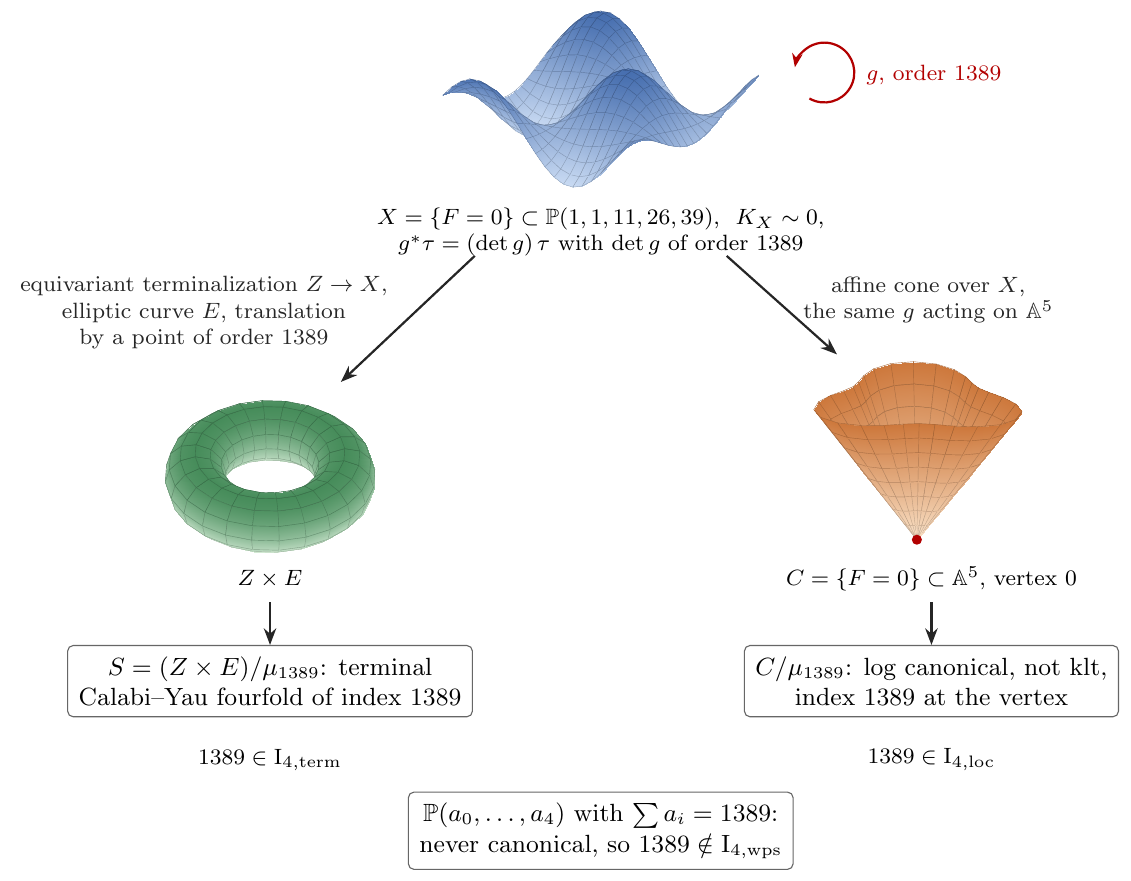
\includegraphics[width=\textwidth]{figures/fig_roadmap.png}
\caption{The plan of the proof. One symmetry $g$ of order $1389$ of the threefold $X$ gives a terminal Calabi--Yau fourfold of index $1389$ (Section~\ref{sec:term}) and a log canonical singularity of index $1389$ (Section~\ref{sec:loc}); no canonical weighted projective fourspace has Fano index $1389$ (Section~\ref{sec:wps}).}
\label{fig:roadmap}
\end{figure}

\begin{remark}\label{rem:literal}
Read literally, $\Il$ contains every positive integer: for $m\geq2$ the group $\mu_m$ acting on $\C^4$ with weights $(1,1,1,m-2)$ is free in codimension one, so $\C^4/\mu_m$ is klt, and $dx_1\wedge\dots\wedge dx_4$ has weight $m+1\equiv1\pmod m$, so its index is $m$ (by the argument in the proof of Proposition~\ref{prop:loc}). Since $3487\notin\Iw$ by \cite[Theorem~4.4]{Liu}, the literal reading fails at once, and the intended reading of $\mathrm{I}_{n,\mathrm{loc}}$ concerns log canonical singularities that are not klt. The singularity of Proposition~\ref{prop:loc} is log canonical and not klt, so Theorem~\ref{thm:main} holds for both readings.
\end{remark}

\section{The threefold}\label{sec:x}

Let $w=(w_0,\dots,w_4)=(1,1,11,26,39)$ and
\[
F=x_0^{77}x_1+x_1^{67}x_2+x_2^{7}x_0+x_3^3+x_4^2\in\C[x_0,\dots,x_4].
\]

\begin{lemma}\label{lem:F}
\begin{enumerate}
\item $F$ is quasi-homogeneous of degree $78=w_0+\dots+w_4$ for the weights $w$.
\item Any three of the $w_i$ are coprime.
\item The partial derivatives of $F$ have no common zero in $\C^5$ other than $0$.
\end{enumerate}
\end{lemma}

\begin{proof}
(1) and (2) are direct. For (3), let $x$ be a common zero; then $x_3=x_4=0$. With $\partial_i=\partial F/\partial x_i$,
\[
x_0\partial_0-77\,x_1\partial_1+5159\,x_2\partial_2=36114\,x_2^7x_0,
\]
since $x_0\partial_0=77x_0^{77}x_1+x_2^7x_0$, $x_1\partial_1=x_0^{77}x_1+67x_1^{67}x_2$ and $x_2\partial_2=x_1^{67}x_2+7x_2^7x_0$. Hence $x_2^7x_0=0$. If $x_2=0$, then $\partial_1=x_0^{77}$ and $\partial_2=x_1^{67}+7x_2^6x_0$ give $x_0=x_1=0$. If $x_0=0$, then $\partial_0=x_2^7$ gives $x_2=0$ and $\partial_2$ gives $x_1=0$.
\end{proof}

Let $C=\{F=0\}\subset\A^5$ and $X=\{F=0\}\subset\PP=\PP(1,1,11,26,39)$. By Lemma~\ref{lem:F}, $X$ is a quasi-smooth hypersurface of degree $78$; $\PP$ and $X$ are well formed \cite[6.10]{IF}. Hence $X$ has cyclic quotient singularities and $\omega_X\cong\mathcal O_X(78-\sum w_i)=\mathcal O_X$ \cite[6.14]{IF}. Quotient singularities are klt \cite[5.20]{KM}, and the discrepancies of a klt variety with Cartier canonical divisor are integers, so $X$ is a canonical Calabi--Yau threefold with $K_X\sim0$.

Fix a primitive $1389$th root of unity $\zeta$ and put $g=\operatorname{diag}(\zeta,\zeta^{1312},\zeta^{992},1,1)$.

\begin{lemma}\label{lem:g}
\begin{enumerate}
\item $F(gx)=F(x)$.
\item $\det g=\zeta^{2305}$ is a primitive $1389$th root of unity.
\item For $0<k<1389$, every fixed point $x\in\C^5$ of $g^k$ has $x_0=x_1=x_2=0$.
\end{enumerate}
\end{lemma}

\begin{proof}
(1) The monomials $x_0^{77}x_1$, $x_1^{67}x_2$ and $x_2^7x_0$ acquire the factors
\[
\zeta^{77+1312}=\zeta^{1389},\qquad\zeta^{67\cdot1312+992}=\zeta^{64\cdot1389},\qquad\zeta^{7\cdot992+1}=\zeta^{5\cdot1389}.
\] (2) $1389=3\cdot463$ and $2305=5\cdot461$ are coprime. (3) The integers $1$, $1312=2^5\cdot41$ and $992=2^5\cdot31$ are prime to $1389$, so $\zeta^k$, $\zeta^{1312k}$ and $\zeta^{992k}$ differ from $1$.
\end{proof}

The matrix $g$ commutes with the $\C^*$-action $t\cdot x=(t^{w_0}x_0,\dots,t^{w_4}x_4)$, so $G=\langle g\rangle\cong\mu_{1389}$ acts on $C$, on $\PP$ and on $X$. Let $\sigma$ be the Poincar\'e residue of $dx_0\wedge\dots\wedge dx_4/F$ along $C$; it generates $\omega_C$, and $g^*\sigma=\det(g)\,\sigma$ by Lemma~\ref{lem:g}(1).

\begin{lemma}\label{lem:omega}
$H^0(X,\omega_X)$ is spanned by a form $\tau$ with $g^*\tau=\det(g)\,\tau$.
\end{lemma}

\begin{proof}
Let $\xi=\sum w_ix_i\,\partial/\partial x_i$ and let $\rho\colon C\setminus\{0\}\to X$ be the quotient map. The $3$-form $\iota_\xi\sigma$ is $\C^*$-invariant, since $\sigma$ has weight $\sum w_i-78=0$, and $\iota_\xi\iota_\xi\sigma=0$. Let $X^\circ\subset X$ be the open set over which $\rho$ is a principal $\C^*$-bundle; its complement has codimension at least $2$ because $X$ is well formed. On $X^\circ$ there is a nowhere vanishing $3$-form $\tau$ with $\rho^*\tau=\iota_\xi\sigma$. As $\omega_X$ is reflexive, $\tau$ is a nowhere vanishing section of $\omega_X\cong\mathcal O_X$, so it spans $H^0(X,\omega_X)$. Since $g$ commutes with $\xi$ and with $\rho$, $g^*\tau=\det(g)\,\tau$.
\end{proof}

\section{A terminal Calabi--Yau fourfold of index 1389}\label{sec:term}

\begin{proposition}\label{prop:term}
$1389\in\It$.
\end{proposition}

\begin{proof}
By \cite[Proposition~2.2]{ETW} there is a $G$-equivariant projective birational morphism $\pi\colon Z\to X$ with $Z$ terminal and $K_Z=\pi^*K_X$. Then $\pi^*\tau$ is a nowhere vanishing section of $\omega_Z$, and $g^*\pi^*\tau=\det(g)\,\pi^*\tau$ by Lemma~\ref{lem:omega}. Let $E$ be an elliptic curve with a point $p$ of order $1389$, and let $G$ act on $Z\times E$ by $g(z,e)=(gz,e+p)$. The action is free, so $S=(Z\times E)/G$ is a terminal projective fourfold and $Z\times E\to S$ is \'etale. With $\eta$ a translation-invariant $1$-form on $E$, the form $\pi^*\tau\wedge\eta$ spans $H^0(Z\times E,\omega_{Z\times E})$ and $g$ multiplies it by $\det(g)$. For $m\geq1$, the sections of $\mathcal O_S(mK_S)$ are the $G$-invariant sections of $\omega_{Z\times E}^{\otimes m}$, so $H^0(S,\mathcal O_S(mK_S))\neq0$ if and only if $\det(g)^m=1$, that is, $1389\mid m$. As $K_S$ is numerically trivial, a nonzero section of $\mathcal O_S(mK_S)$ has no zeros, so $mK_S\sim0$ exactly when $1389\mid m$. This is the argument of \cite[Corollary~4.1]{ETW}. Hence $S$ is a terminal Calabi--Yau fourfold of index $1389$.
\end{proof}

\section{A log canonical singularity of index 1389}\label{sec:loc}

\begin{lemma}\label{lem:cone}
$C$ is normal and Gorenstein, log canonical, and not klt.
\end{lemma}

\begin{proof}
By Lemma~\ref{lem:F}(3), $C$ is a hypersurface whose only singular point is $0$, so $C$ is Gorenstein and, by Serre's criterion, normal; its local ring at $0$ is a domain, so $C$ is irreducible and no coordinate $x_j$ divides $F$.

Let $B\to\A^5$ be the weighted blow-up of $0$ with weights $w$. It is covered by the charts $U_i=\A^5/\mu_{w_i}$, where $\varphi_i\colon\A^5_y\to\A^5_x$ is $x_i=y_i^{w_i}$, $x_j=y_jy_i^{w_j}$ ($j\neq i$), and $\varepsilon\in\mu_{w_i}$ acts by $y_i\mapsto\varepsilon y_i$, $y_j\mapsto\varepsilon^{-w_j}y_j$. Quasi-homogeneity gives $F\circ\varphi_i=y_i^{78}F_i$, where $F_i$ is $F$ with $x_i$ replaced by $1$ and $x_j$ by $y_j$; it does not involve $y_i$. Let $S_i=\{F_i=0\}$ in the coordinates $y_j$, $j\neq i$. If $F_i$ and its derivatives vanish at $u$ (with $u_i=1$), the Euler identity $78F=\sum w_jx_j\partial_jF$ gives $\partial_iF(u)=0$, contradicting Lemma~\ref{lem:F}(3); so $S_i$ is smooth. The strict transform $W$ of $C$ is covered by $W_i=V_i/\mu_{w_i}$ with $V_i=\A^1_{y_i}\times S_i$, and the exceptional divisor $E_W=W\cap\pi^{-1}(0)$ is covered by $D_i/\mu_{w_i}$ with $D_i=\{0\}\times S_i$.

The action of $\mu_{w_i}$ on $V_i$ is free in codimension one. A non-identity $\varepsilon$ fixes no point with $y_i\neq0$. Its fixed points in $D_i$ satisfy $y_j=0$ for some $j\neq i$ with $\varepsilon^{w_j}\neq1$, which exists because the $w_j$ with $j\neq i$ are coprime; and $\{y_j=0\}$ contains no component of $S_i$ because $x_j\nmid F$. Hence $q_i\colon V_i\to W_i$ is \'etale in codimension one, $q_i^*K_{W_i}=K_{V_i}$ and $q_i^*E_W=D_i$. The pair $(V_i,D_i)$ is a smooth variety with a smooth divisor, hence log canonical, so $(W,E_W)$ is log canonical by \cite[5.20]{KM}.

The Jacobian of $\varphi_i$ is $w_iy_i^{\sum w_j-1}$, so
\[
\varphi_i^*(dx/F)=w_iy_i^{\sum w_j-1-78}\,dy/F_i=w_iy_i^{-1}\,dy/F_i,
\]
and the pullback of $\sigma$ to $V_i$ is $w_iy_i^{-1}$ times a generator of $\omega_{V_i}$. Thus the pullback of $\sigma$ to $W$ is a rational section of $\omega_W$ with divisor $-E_W$, that is, $K_W+E_W=\psi^*K_C$ for $\psi\colon W\to C$. By \cite[Lemma~2.30]{KM}, every divisor over $C$ has the same discrepancy for $C$ as for $(W,E_W)$. So $C$ is log canonical, and $E_W$ has discrepancy $-1$, so $C$ is not klt.
\end{proof}

\begin{figure}[ht]
\centering
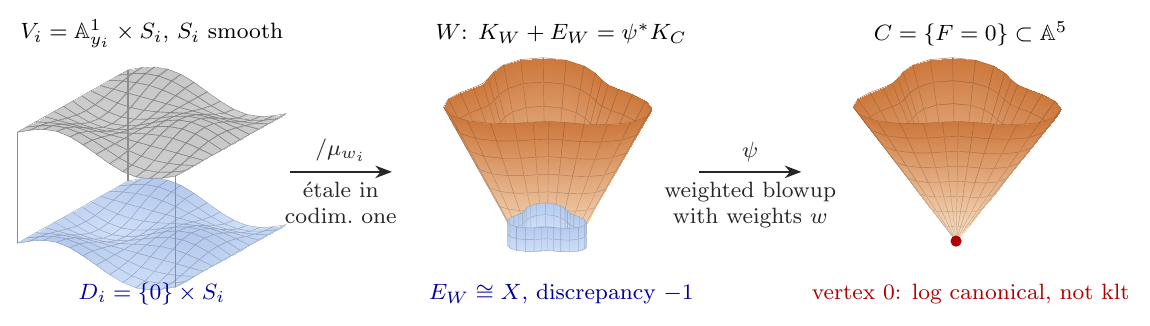
\includegraphics[width=\textwidth]{figures/fig_blowup.png}
\caption{The proof of Lemma~\ref{lem:cone}. The weighted blowup $\psi$ replaces the vertex of $C$ by $E_W\cong X$, and $K_W+E_W=\psi^*K_C$. On the chart $V_i$ the pair $(V_i,D_i)$ is a smooth variety with a smooth divisor, and $V_i\to W_i$ is a quotient by $\mu_{w_i}$ that is \'etale in codimension one.}
\label{fig:blowup}
\end{figure}

\begin{proposition}\label{prop:loc}
Let $Y=C/G$ and let $P\in Y$ be the image of $0$. Then $P\in Y$ is a four-dimensional log canonical singularity that is not klt and has index $1389$. In particular, $1389\in\Il$.
\end{proposition}

\begin{proof}
By Lemma~\ref{lem:g}(3), the fixed locus of $g^k$ on $C$ for $0<k<1389$ lies in the curve $\{x_0=x_1=x_2=0,\ x_3^3+x_4^2=0\}$. So $p\colon C\to Y$ is \'etale in codimension one, $K_C=p^*K_Y$, and $Y$ is log canonical and not klt by Lemma~\ref{lem:cone} and \cite[5.20]{KM}.

For $m\geq1$, the sections of $\mathcal O_Y(mK_Y)$ near $P$ are the $G$-invariant sections of $\omega_C^{\otimes m}$, that is, $f\sigma^m$ with $g^*f=\det(g)^{-m}f$. If $1389\mid m$, then $\sigma^m$ is invariant and generates. Conversely, if $mK_Y$ is Cartier at $P$ with generator $f\sigma^m$, then $f(0)\neq0$, and $g(0)=0$ gives $f(0)=\det(g)^{-m}f(0)$, so $1389\mid m$ by Lemma~\ref{lem:g}(2).
\end{proof}

\section{Weighted projective spaces of Fano index 1389}\label{sec:wps}

For $a=(a_0,\dots,a_4)\in\Z_{>0}^5$ with $q=\sum a_i$ and $k\in\Z$, put
\[
\age_a(k)=\sum_{i=0}^4\Big\{\frac{ka_i}{q}\Big\}=k-\sum_{i=0}^4\Big\lfloor\frac{ka_i}{q}\Big\rfloor.
\]
By Kasprzyk's criterion \cite[Proposition~2.5]{Kas}, a well-formed $\PP(a)$ has canonical singularities if and only if $\age_a(k)\in\{1,2,3\}$ for every $k\in\{2,\dots,q-2\}$.

\begin{lemma}\label{lem:witness}
Let $a\in\Z_{>0}^5$, $q=\sum a_i$, $k\in\Z$, and let $r_i\in\{0,\dots,q-1\}$ be the residue of $ka_i$ modulo $q$. If $r_i\geq1$ for $i=1,2,3,4$ and $r_1+r_2+r_3+r_4\leq q-1$, then $\age_a(q-k)=4$.
\end{lemma}

\begin{proof}
Since $\sum ka_i=kq$, we have $r_0\equiv-(r_1+\dots+r_4)\pmod q$, and $1\leq r_1+\dots+r_4\leq q-1$ gives $r_0=q-(r_1+\dots+r_4)\geq1$. All five residues are positive, so $\{(q-k)a_i/q\}=1-r_i/q$ and $\age_a(q-k)=5-\sum r_i/q=4$.
\end{proof}

\begin{proposition}\label{prop:cert}
Let $q=1389$. For all integers $1\leq a_4\leq a_3\leq a_2\leq a_1$ with $2a_1+a_2+a_3+a_4\leq q$ there is $k\in\{2,\dots,q-2\}$ such that the residues $r_i$ of $ka_i$ modulo $q$ satisfy $r_1,\dots,r_4\geq1$ and $r_1+r_2+r_3+r_4\leq q-1$.
\end{proposition}

\begin{proof}
The proof is a finite verification, carried out in the Lean kernel (Section~\ref{sec:lean}). For $t=(t_1,\dots,t_4)$ with $t_4\leq t_3\leq t_2\leq t_1$ let $x_i=1+8t_i$ and let $Q_t$ be the box $\prod_i\{x_i,\dots,x_i+7\}$. Every admissible $(a_1,\dots,a_4)$ lies in $Q_t$ for $t_i=\lfloor(a_i-1)/8\rfloor$, and then $2x_1+x_2+x_3+x_4\leq q$. There are $368{,}253$ such $t$. For each of them the certificate lists values of $k$, $2{,}624{,}293$ in all and at most $70$ per box; one value suffices for $231{,}139$ boxes. The condition on $k$ is equivalent to
\begin{equation}\label{eq:test}
\sum_{i=1}^4\big(((ka_i+q-1)\bmod q)+1\big)\leq q-1,
\end{equation}
because $((ka+q-1)\bmod q)+1$ equals the residue of $ka$ when that residue is positive and equals $q$ otherwise. Write $a_i=x_i+\delta_i$ with $0\leq\delta_i\leq7$ and $c_i=(kx_i+q-1)\bmod q$. Then $(ka_i+q-1)\bmod q=c_i+k\delta_i-q\lfloor(c_i+k\delta_i)/q\rfloor$ and
\[
\Big\lfloor\frac{c_i+k\delta_i}{q}\Big\rfloor=\#\Big\{j\geq1:\ \delta_i\geq\Big\lceil\frac{jq-c_i}{k}\Big\rceil\Big\},
\]
a sum of at most $\lfloor(c_i+7k)/q\rfloor$ indicator functions of $\delta_i$. The checker stores the $8^4$ points of a box in $17$-bit fields of one natural number and evaluates \eqref{eq:test}, the order conditions and the linear condition for all of them by additions, multiplications by integers, shifts and bitwise conjunctions; a box passes when every admissible point satisfies \eqref{eq:test} for some listed $k$. The soundness of the checker, namely that a passing box has this property, is proved in Lean, and the kernel evaluates the checker on all boxes.
\end{proof}

\begin{figure}[ht]
\centering
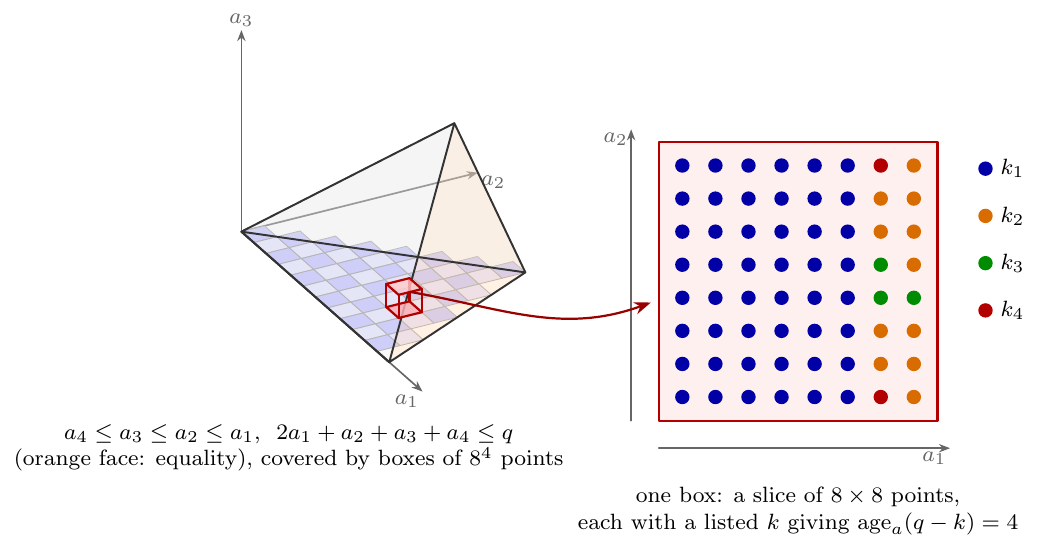
\includegraphics[width=\textwidth]{figures/fig_boxes.png}
\caption{The certificate of Proposition~\ref{prop:cert}. The sorted weights with $2a_1+a_2+a_3+a_4\leq q$ are covered by boxes of $8^4$ points (drawn in the coordinates $a_1,a_2,a_3$). For each box the certificate lists values of $k$; every point of the box is served by one of them. The right panel shows the points of one slice of one box, coloured by the listed value that serves them.}
\label{fig:boxes}
\end{figure}

\begin{theorem}\label{thm:wps}
Every $a\in\Z_{>0}^5$ with $\sum a_i=1389$ has $\age_a(k)=4$ for some $k\in\{2,\dots,1387\}$. Hence no well-formed weighted projective space $\PP(a_0,\dots,a_4)$ of Fano index $1389$ has canonical singularities, and $1389\notin\Iw$.
\end{theorem}

\begin{proof}
Order the weights so that $a_0\geq a_1\geq\dots\geq a_4$. Then $2a_1+a_2+a_3+a_4\leq a_0+\dots+a_4=1389$. Proposition~\ref{prop:cert} gives $k\in\{2,\dots,1387\}$, and Lemma~\ref{lem:witness} gives $\age_a(1389-k)=4$ with $1389-k\in\{2,\dots,1387\}$. Kasprzyk's criterion excludes canonical singularities, and $1389>4$.
\end{proof}

\begin{proof}[Proof of Theorem~\textup{\ref{thm:main}}]
Combine Propositions~\ref{prop:term} and~\ref{prop:loc} with Theorem~\ref{thm:wps}.
\end{proof}

\begin{remark}
Since $\varphi(1389)=924\leq984$, the number $1389$ lies in the set $\{m:\varphi(m)\leq984\}$ that contains $\Iw$ by \cite[Theorem~4.4]{Liu}; it is one of the elements of the set $\mathrm J_4$ of \cite[Section~4]{Liu}. Theorem~\ref{thm:wps} agrees with the list \cite{LiuData}. The neighbouring index $1383$ lies in $\Iw$: $\PP(674,461,195,35,18)$ is well formed and passes Kasprzyk's criterion.
\end{remark}

\section{Formal verification}\label{sec:lean}

The finite and algebraic parts of the proof are formalized in Lean~4 with its mathematical library \cite{Lean,Mathlib}. In the formalization the set $\Iw$ is defined as the union of $\{1,2,3,4\}$ with the sums $\sum a_i$ over the well-formed $a\in\Z_{>0}^5$ that satisfy Kasprzyk's criterion. The formal statements are Lemma~\ref{lem:F}, Lemma~\ref{lem:g}, Proposition~\ref{prop:cert}, the first part of Theorem~\ref{thm:wps}, and the statement $1389\notin\Iw$. The kernel checks every proof, and each of these theorems depends only on the axioms of propositional extensionality, choice and quotient soundness.

The certificate of Proposition~\ref{prop:cert} is split into $4{,}022$ statements, each asserting that the checker accepts one list of boxes. Each statement is closed by evaluating the checker in the kernel, so no compiled code is trusted; checking all of them takes about $15$ minutes on four cores. The steps that rest on the literature, namely Kasprzyk's criterion, the results of \cite{IF} and \cite{ETW}, and the singularity theory of Sections~\ref{sec:x}--\ref{sec:loc}, are proved in the text and not formalized, since the library does not yet contain weighted projective spaces or discrepancies.

Independently of the formalization, programs in C, C++, Julia and Python enumerate all $1{,}301{,}769{,}806$ partitions of $1389$ into five parts, test Kasprzyk's criterion on the $874{,}763{,}737$ well-formed ones, and find no canonical one. The same enumeration for $q=1383$ finds $\PP(674,461,195,35,18)$.

\section*{Acknowledgements}
The authors used the generative AI tool Claude (Anthropic), through Claude Code, to assist with the proofs, the Lean formalization, the computations and the preparation of this article. The authors reviewed and edited the content and take full responsibility for it.

\section*{Competing interests}
None.

\section*{Funding}
None.

\section*{Data availability}
\begingroup\raggedright
\ifanon
The computations and the Lean formalization were carried out by the authors with the help of AI assistance (Claude, Anthropic). The Lean formalization, the certificate generator and the search programs are supplied with the submission.\par
\else
Deep Bhattacharjee computed the Lean formalization and the Julia, C, C++, shell and Python computations with the help of AI assistance (Claude, Anthropic). The Lean formalization of the finite and algebraic parts of the proof, together with the certificate generator and the search programs, is archived at Zenodo \cite{archive}, doi:\href{https://doi.org/\zenodoID}{\zenodoID}. The paper is available at \url{\preprintURL}.\par
\fi
\endgroup

\begin{thebibliography}{99}
\raggedright

\ifanon\else
\bibitem{archive}
D.~Bhattacharjee and U.~Bhattacharya, \emph{A counterexample to Liu's conjecture on Fano indices in dimension four: Lean formalization and programs}, Zenodo, 2026, doi:\href{https://doi.org/\zenodoID}{\zenodoID}.
\fi

\bibitem{Mathlib}
The mathlib Community, \emph{The Lean mathematical library}, in: Proceedings of the 9th ACM SIGPLAN International Conference on Certified Programs and Proofs (CPP 2020), ACM, 2020, pp.~367--381, doi:\href{https://doi.org/10.1145/3372885.3373824}{10.1145/3372885.3373824}.

\bibitem{ETW}
L.~Esser, B.~Totaro and C.~Wang, \emph{Calabi--Yau varieties of large index}, Algebr. Geom., to appear; arXiv:2209.04597.

\bibitem{IF}
A.~R.~Iano-Fletcher, \emph{Working with weighted complete intersections}, in: Explicit birational geometry of 3-folds, London Math. Soc. Lecture Note Ser. 281, Cambridge Univ. Press, Cambridge, 2000, pp.~101--174, doi:\href{https://doi.org/10.1017/CBO9780511758942.005}{10.1017/CBO9780511758942.005}.

\bibitem{Kas}
A.~M.~Kasprzyk, \emph{Classifying terminal weighted projective space}, arXiv:1304.3029.

\bibitem{KM}
J.~Koll\'ar and S.~Mori, \emph{Birational geometry of algebraic varieties}, Cambridge Tracts in Math. 134, Cambridge Univ. Press, Cambridge, 1998, doi:\href{https://doi.org/10.1017/CBO9780511662560}{10.1017/CBO9780511662560}.

\bibitem{Liu}
H.~Liu, \emph{On Fano indices of weighted projective spaces}, arXiv:2608.03434v3, 2026.

\bibitem{LiuData}
H.~Liu, \emph{Fano indices of four-dimensional canonical weighted projective spaces} (data and code), Zenodo, doi:\href{https://doi.org/10.5281/zenodo.21806548}{10.5281/zenodo.21806548}.

\bibitem{Lean}
L.~de~Moura and S.~Ullrich, \emph{The Lean~4 theorem prover and programming language}, in: Automated Deduction -- CADE 28, Lecture Notes in Comput. Sci. 12699, Springer, 2021, pp.~625--635, doi:\href{https://doi.org/10.1007/978-3-030-79876-5_37}{10.1007/978-3-030-79876-5\_37}.

\end{thebibliography}

\end{document}
